% !TEX program = xelatex
\documentclass{mcmthesis}
\mcmsetup{CTeX =false,   % 使用 CTeX 套装时,设置为 true
        tcn = 2113633, problem = A,
        sheet = true, titleinsheet =true, keywordsinsheet = true,
        titlepage =false, abstract = false}
\usepackage{palatino}
\usepackage{lipsum}
\usepackage{times}
\usepackage{geometry}
\usepackage{float}
\usepackage{diagbox}
\usepackage{multicol}
\usepackage{setspace}
% \usepackage{ctex}
%===============设置正文和数学字体=============================
%有些字体需要安装一些字体文件,注意辨别。


\usepackage{graphicx}
\usepackage{subfigure}
%设置段落之间的距离,若不需要删除或者注释掉即可。
\setlength\parskip{.5\baselineskip}
\newtheorem{definition}{Definition}[section]
%\def\abstractname{Summary}%可修改摘要名称

\usepackage{indentfirst}
\setlength{\parindent}{2em}

\usepackage{chngpage}
\usepackage{array}
\usepackage{booktabs}
\usepackage{threeparttable}
\usepackage{longtable}
\usepackage[numbers,sort&compress]{natbib}
%%% 实现参考文献标号在右上角
\newcommand{\upcite}[1]{\textsuperscript{\textsuperscript{\cite{#1}}}}
%然后引用的时候使用\upcite{}的格式(一般的正常引用格式为\cite{})

\usepackage{titletoc}
\titlecontents{section}[3cm]{\bf \large}{\contentslabel{2.8em}}{}{%
\titlerule*[0.5pc]{$\cdot$}\contentspage}%
\titlecontents{subsection}[4cm]{\normalsize}{\contentslabel{2.5em}}{}{%
\titlerule*[0.5pc]{$\cdot$}\contentspage}%
\titlecontents{subsubsection}[5.3cm]{\normalsize}{\contentslabel{3.0em}}{}{%
\titlerule*[0.5pc]{$\cdot$}\contentspage}%

\title{\large Research on the decomposition of fungi and related environmental problems}
\author{ }

\date{\today}

\geometry{left=3.0cm,right=3.0cm}

\linespread{1}

\begin{document}
\begin{abstract}
    
In order to analyze the decomposition of woody fibers in fungal community, this paper deduces the competitive formula applicable to multi-fungal community from the relevant theory, and regards this problem as a problem of multi-interaction and coexistence between populations based on competition. We establish and optimize the relationship between populations, focus on analyzing the stability of the model, and finally simulate the relationship between fungal community, diversity and the influence of environmental condition fluctuation on the overall rate decomposition of fungi reasonably. The stable conditions of the system are determined theoretically.

For problem 1 and 2, we use the linear fitting method, and show the effect of different arguments on the rate of fungal decomposition as a function. For the two most important variables, Hyphal extension and moisture trade-off. By researching the relevant images, we carry out linear and nonlinear fitting method, obtain the relationship and merge them .

For problem 3, we refine our model based on the Lotuka-Voltera model, and the relationship between different fungi is expressed through the different equations. To solve the singerum characteristics and types and analyze the stability and stable conditions of the model, we finally give an analysis of the two fungal community as examples and list the competitive results under different circumstances. It is concluded that when the two sides only have a competitive relationship, the two will eventually achieve relative stability in quantity. However, if there is a suppression relationship, there will be a situation in which one of the winning parties is eliminated.

For problem 4, which based on the model of problem 3, the effects of dynamic fluctuations are added to simulate short-term changes in different environments such as drought, semi-arid, temperate, trees and tropical rainforests. We analyze the stability of the power system in the presence of dynamic interference, and divide the results of each fungus into four cases: “extinction”, “average persistent”, “weakly average persistent”, and “strongly average persistent” according to relevant definitions. Furthermore we analyze the each situation needs to meet the conditions.

For problem 5, in order to simulate fungal diversity, which includes competition, inhibition, promotion and the existence of three interrelations at the same time, we optimize the model further taking the three fungal coexistence as an example. We use the matrix to analyze the diversity system, so the conditions of the positive equilibrium point of global progressive stability are clearly expressed in matrix form, which describes the important influence of fungal diversity on ecosystem stability and system self-regulation ability. Finally, the overall decomposition rate of wood fibers of the diversity fungus system is solved by combining the models of problem 1 and 2.

\begin{keywords}
    The decomposition rate of fungi, Stability analysis, Ecosystem diversity, Competition-inhibition-promotion mixed relationship model, Dynamic system, Random disturbance
\end{keywords}
\end{abstract}
\maketitle
    
\begin{adjustwidth}{-1cm}{0cm}
    
    \setcounter{tocdepth}{3}
    \thispagestyle{empty}
    \begin{spacing}{0.9}
    \tableofcontents
    \end{spacing}
    
    \end{adjustwidth}
\pagestyle{fancy}
\setcounter{page}{1}
\section{Introduction}
    \subsection{Background}
Ecosystem is an open system, both material and energy are constantly circulating and exchanging with the outside world. The cycle of matter and energy requires the joint efforts of producers and decomposers. Producers gather matter and energy in the system, while decomposers release them, which is crucial to the balance and development of the entire ecosystem. The diversity of fungi in the ecosystem is very rich and it plays an important role in maintaining the stability of the diversity of the ecosystem.It is of great significance and influence to study the development of the whole ecosystem to systematically study the decomposition models of fungi and analyze their roles in the ecosystem.

    \subsection{Restatement of the Problems}
\begin{itemize}
\item[$\bullet$] Build a mathematical model that describes the breakdown of ground litter and woody fibers through fungal activity in the presence of multiple species of fungi.
\item[$\bullet$] In your model, incorporate the interactions between different species of fungi, which have different growth rates and different moisture tolerances.

\item[$\bullet$] Provide an analysis of the model and describe the interactions between the different types of fungi. 

\item[$\bullet$] Include predictions about the relative advantages and disadvantages for each species and combinations of species likely to persist, and do so for different environments.

\item[$\bullet$] Describe how the diversity of fungal communities of a system impacts the overall efficiency of a system with respect to the breakdown of ground litter. Predict the importance and role of biodiversity in the presence of different degrees of variability in the local environment.
\end{itemize}





    
\pagestyle{fancy}
\section{Analysis of the Problems}
    \subsection{Analysis of the Problem 1}
We need to establish a "decomposition rate model", which focuses on describing the breakdown of ground litter and woody fibers through fungal activity in the presence of multiple species of fungi. In the process of building the model, we need to consider the influence of woody plant species, site, years decayed, mesh, sampling side, extension rate, temperature, humidity overlap degree, time and other independent variables that may affect the decomposition process on the decomposition rate, and take the decomposition rate as the dependent variable for fitting.
    \subsection{Analysis of the Problem 2}
According to the research results of Nicky Lustenhouwer et al\upcite{Lustenhouwer11551}. in the attachment, it can be concluded that both the hyphal extension rate and the moisture trade-off are related to the decomposition rate, and there are specific interactions between them. To solve this question, we need to establish a model to combine these two interactions, and optimize the model by using the functional relationship between them while keeping the decomposition rate unchanged.

    \subsection{Analysis of the Problem 3}
In the same living environment, space and resources are limited, so the interaction between different types of fungi is usually manifested as competition relationship, that is, competition between different populations. In this question, a dynamic interaction model based on Logistic model and Lotka-Voltrra model should be established, and the influence of atmospheric environment such as temperature and humidity on the interaction between different types of fungi should be realized by controlling the growth rate, the degree of inhibition, the environmental tolerance and other coefficients.
    \subsection{Analysis of the Problem 4}
This question needs to predict the relative advantages and disadvantages of possible species combinations and make reasonable predictions for different environments. Therefore, the influence of "dynamic fluctuations" can be considered on the basis of the model established in problem 3. We can add random disturbance factors and introduce a random population model to simulate the effects of different environments on the fungal population.

    \subsection{Analysis of the Problem 5}
In order to describe how the diversity of fungal communities of a system impacts the overall efficiency of a system with respect to the breakdown of ground litter, it is necessary to consider the changes when different interactions (not only competition) between fungal communities coexist on the basis of the dynamic interaction model of the third question, analyze the relationship between the number of fungal species and decomposition efficiency, and simulate the variability of local environment by setting initial conditions.
    
\pagestyle{fancy}
\section{Assumptions}

To simplify the problem, we make the following basic assumptions, each of which is properly justified.

\begin{itemize}
    \item[$\bullet$] Nutrients such as ground litter and woody fibers are only broken down by fungi and not broken down or consumed by other organisms.
    \item[$\bullet$] The maximum environmental capacity of the fungal community is constant over a period of time and only depends on the size of space and the amount of resources.
    \item[$\bullet$] After a fungus has been eliminated from the competition, it is likely to reappear if environmental conditions change.
    \item[$\bullet$] Even when different communities are not in direct contact, they are competing and interacting with each other all the time.
\end{itemize}
    
\pagestyle{fancy}
\newpage
\section{Symbol Description}
\renewcommand\arraystretch{1.2}
\begin{center}
    \begin{longtable}{|c|l|}
    \caption{The List of Symbol Description}\\ \hline
    Symbol & Description \\ \hline

    $y$  & decomposition rate \\ \hline

    $x_{i}$ & the value of the i-th influencing factor \\ \hline

    $h$ & the hyphal extension rate \\ \hline

    $m$ & moisture trade-off \\ \hline

    $N$ & the size (expressed in number) of fungi \\ \hline

    $K$ & the maximum environmental tolerance of fungi \\ \hline

    $r$ & the growth rate of fungi \\ \hline

    \end{longtable}

    \end{center}
\pagestyle{fancy}
\section{Model Establishment and Solution of Problem}
    \subsection{Problem 1}
\subsubsection{Decomposition rate model}

By consulting relevant data and analyzing, it can be found that the main factors affecting the decomposition rate include temperature, humidity, overlap degree between communities, oxygen concentration, illumination intensity, time, woody plant species, site, years decayed, mesh, sampling side, extension rate, etc. Therefore, we can take the above influencing factors as independent variables, and choose the decomposition rate as the dependent variable to describe the breakdown of ground litter and woody fibers, and start to establish the decomposition rate model.

It is assumed that there are $k$ independent variables. Firstly, each independent variable is quantified, normalized and dimensionless, and the category variable needs dummy element processing. Then, in the case of known data of $N$ groups of $k$ independent variables, the decomposition rate's approximate equation of each independent variable is selected as follows:
\begin{equation}\label{1.1}
    y^{*}=a_{0}+a_{1}x_{1}+\dots+a_{k}x_{k}
\end{equation}
Where,

$y^{*}$ is the approximate value of $y$;

$x_{i}$ is the value of the i-th influencing factor, namely the i-th independent variable;

$a_{i}$ is the assumed coefficient, $i=0, 1, \dots, k$.

In the case of known data of $N$ groups of $k$ independent variables, the minimum sum of squares of the deviation between the measured value and the calculated value is taken as the "optimization criterion". Let:
\begin{equation}\label{1.2}
    \varphi(a_{0},a_{1},\dots\,a_{k})=\sum_{n = 1}^{N}(y_{n}-y_{n}^{*})^{2}=\sum_{n = 1}^{N} (y_{n}-a_{0}-a_{1}x_{1n}-\dots-a_{k}x_{kn})^{2}
\end{equation}

Where,

$y_{n}$ is the decomposition rate under the data of the nth group;

$y_{n}^*$ is the approximate value of the decomposition rate under data of the nth group;

$x_{in}$ is the ith independent variable under the data of the nth group.

The least square method is used to determine all the coefficients in Equation (\ref{1.1}):

Through the method of finding the extreme value of the multivariate function, take the partial derivative in Equation (\ref{1.2}) and make it equal to zero, so as to reach the minimum value. For $k+1$ partial derivatives are as follows:
\begin{equation}\label{}
\left\{
\begin{array}{l}
    \frac{\partial \varphi}{\partial a_{0}} = -2\sum_{n = 1}^{N} (y_{n}-a_{0}-a_{1}x_{1n}-\dots-a_{k}x_{kn})=0 \\
    \frac{\partial \varphi}{\partial a_{1}} = -2\sum_{n = 1}^{N} (y_{n}-a_{0}-a_{1}x_{1n}-\dots-a_{k}x_{kn})x_{1n}=0 \\
    \dots \\
    \frac{\partial \varphi}{\partial a_{k}} = -2\sum_{n = 1}^{N} (y_{n}-a_{0}-a_{1}x_{1n}-\dots-a_{k}x_{kn})x_{kn}=0 \\
\end{array}
\right.
\end{equation}

By transforming the above equation, we get:
\begin{equation}\label{}
\left\{
\begin{array}{l}
    Na_{0}+\sum_{n = 1}^{N}a_{1}x_{1n}+\dots+\sum_{n = 1}^{N}a_{k}x_{kn}=\sum_{n = 1}^{N}y_{n} \\

    \sum_{n = 1}^{N}a_{0}x_{1n}+\sum_{n = 1}^{N}a_{1}x_{1n}x_{1n}+\dots+\sum_{n = 1}^{N}a_{k}x_{kn}x_{1n}=\sum_{n = 1}^{N}y_{n}x_{1n} \\

    \dots \\

    \sum_{n = 1}^{N}a_{0}x_{kn}+\sum_{n = 1}^{N}a_{1}x_{1n}x_{kn}+\dots+\sum_{n = 1}^{N}a_{k}x_{kn}x_{kn}=\sum_{n = 1}^{N}y_{n}x_{kn} \\
\end{array}
\right.
\end{equation}

After further simplification, we can get:
\begin{equation}\label{1.4}
\left\{
\begin{array}{l}
    a_{1}l_{11}+a_{2}l_{12}+\dots+a_{k}l_{1k}=l_{1y} \\
    a_{1}l_{21}+a_{2}l_{22}+\dots+a_{k}l_{2k}=l_{2y} \\
    \dots \\
    a_{1}l_{k1}+a_{2}l_{k2}+\dots+a_{k}l_{kk}=l_{ky} \\
\end{array}
\right.
\end{equation}

\begin{equation}\label{1.5}
    a_{0}=\bar{y}-a_{1}\bar{x_{1}}-\dots-a_{k}\bar{x_{k}}
\end{equation}

Where,
\begin{equation}\label{}
\left\{
\begin{array}{l}
    l_{ij}=l_{ji}=\sum_{n = 1}^{N}x_{in}x_{jn}-\frac{1}{N}(\sum_{n = 1}^{N}x_{in})(\sum_{n = 1}^{N}x_{jn})  \\
    l_{iy}=\sum_{n = i}^{N}y_{n}x_{in}-\frac{1}{N}(\sum_{n = 1}^{N}x_{in})(\sum_{n = 1}^{N}x_{jn})  \\
    i=1,2,\dots,k; j=1,2,\dots,k; \\
\end{array}
\right.
\end{equation}

According to the above transformation, as long as the relevant variables satisfy the Equation (\ref{1.4}) and Equation (\ref{1.5}), the minimum value of $\varphi (a_{0},a_{1},\dots,a_{k})$ can be obtained. So we can determine all the coefficients by solving Equation (\ref{1.4}) and Equation (\ref{1.5}). Then, the decomposition rate can be obtained as follows:

\begin{equation}\label{}
    y=f(x_{1},x_{2},\dots,x_{k})=a_{0}+a_{1}x_{1}+\dots+a_{k}x_{k}
\end{equation}

\subsubsection{Solution of Problem 1}

By analyzing the data provided by Nicky Lustenhouwer\upcite{Lustenhouwer11551}, we draw four violin maps to analyze the relationship between the Mass loss and Site, Years decayed, Mesh and Sampling side.
\begin{figure}[H]
    \centering
    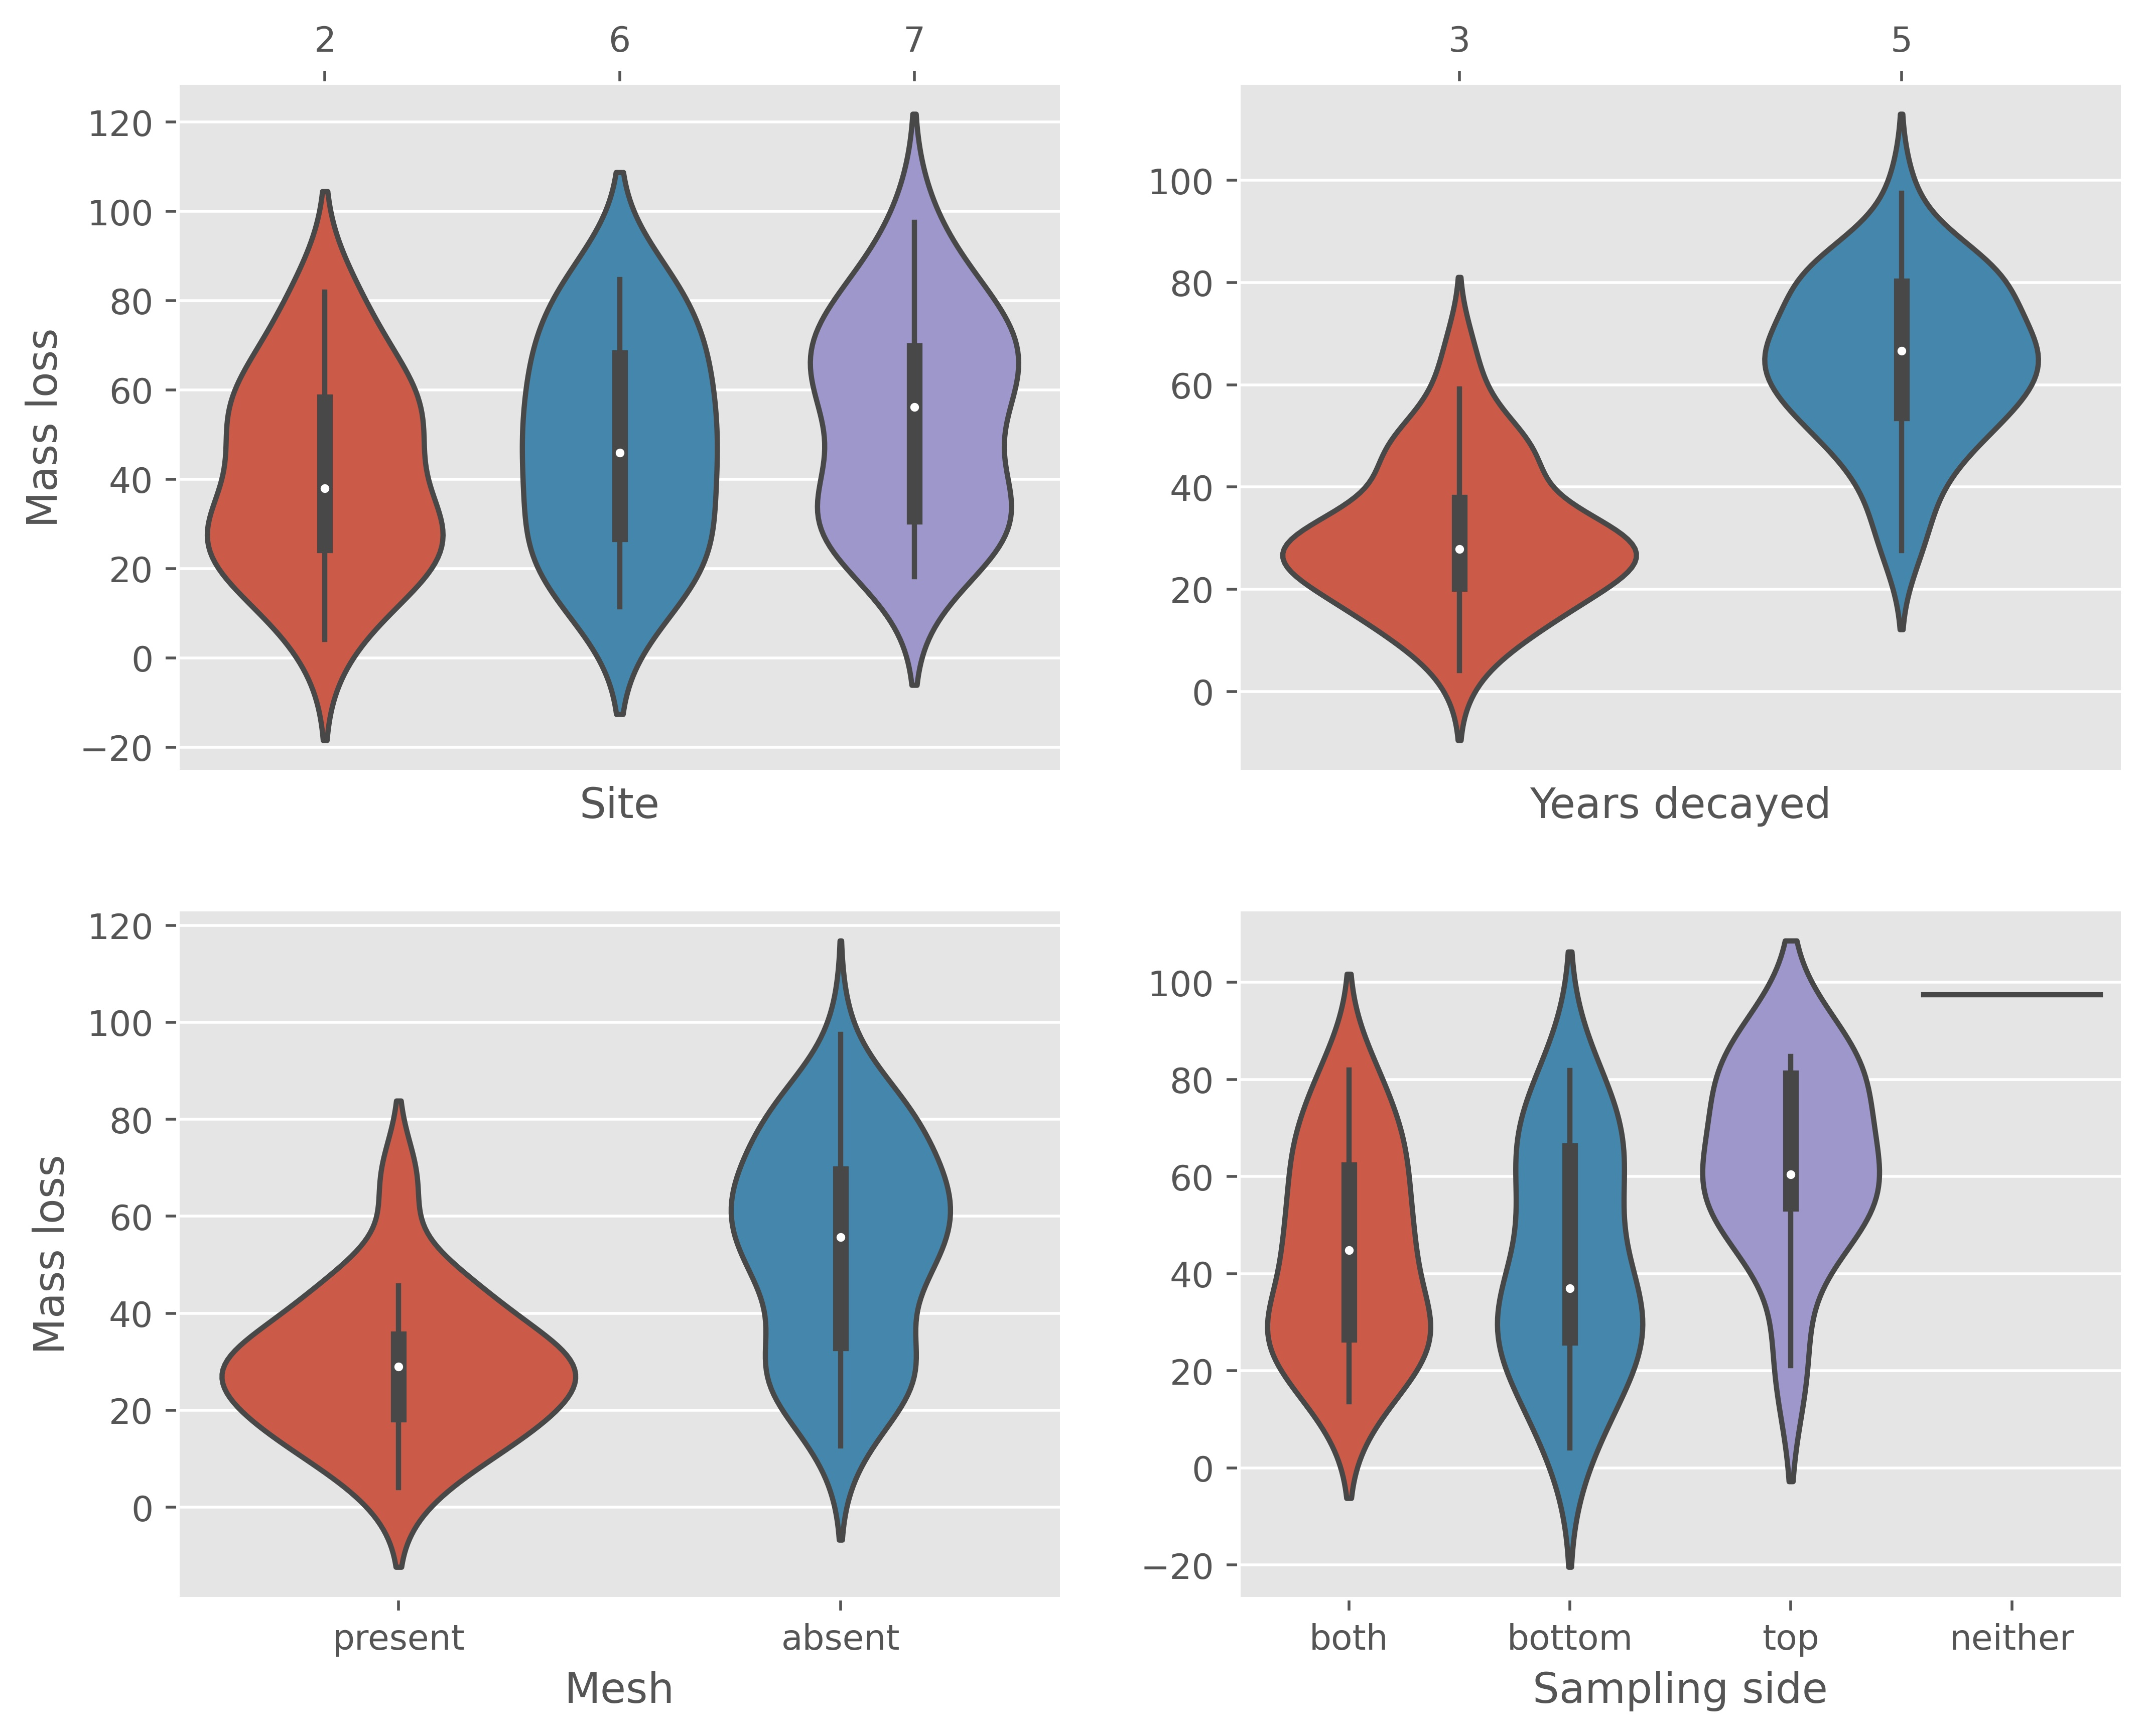
\includegraphics[width=0.6\textwidth]{./code/fig1.jpg}
    \caption{Violin maps between Mass loss and other variables}\label{fig1}
\end{figure}

Among the four maps showed in Figure (\ref{fig1}), we can find clearly the close connection between Mass loss and Years decayed. So we explore the linear relationship between Mass loss and Extension rate grouped by Years decayed as follows:
\begin{figure}[H]
    \centering
    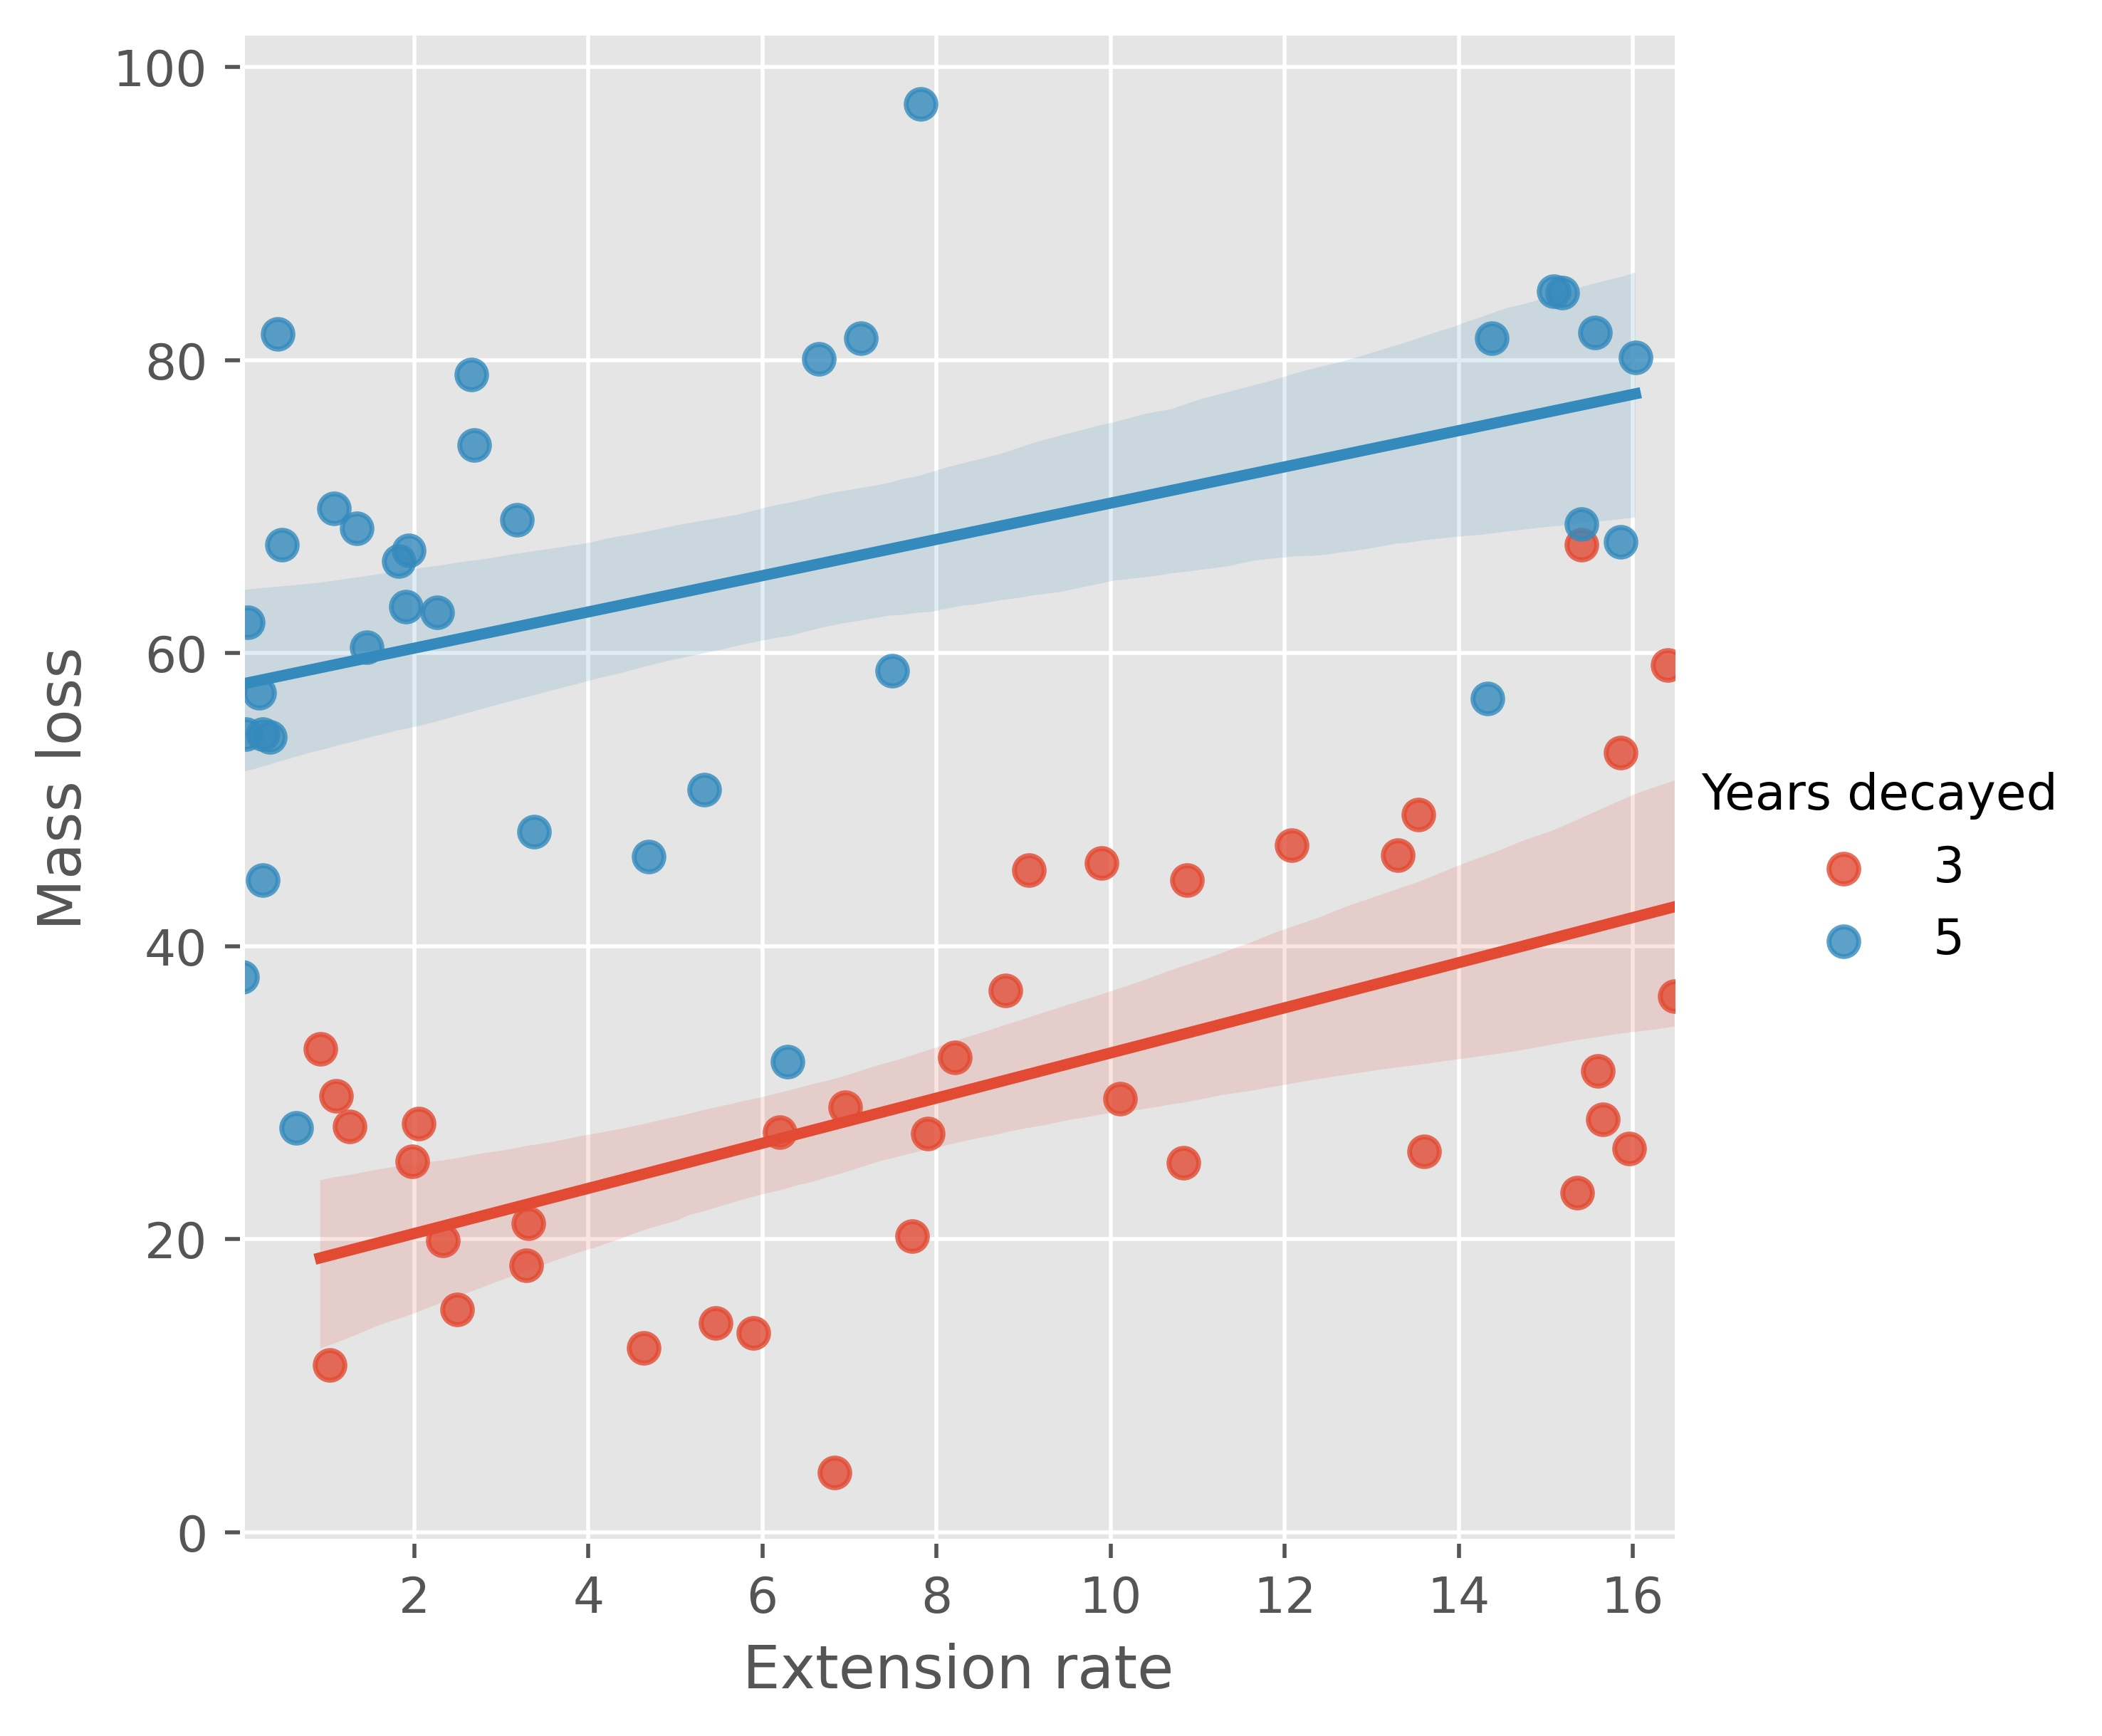
\includegraphics[width=0.65\textwidth]{./code/fig2.jpg}
    \caption{Linear relationship between Mass loss and Extension rate}\label{fig2}
\end{figure}

Using the least square method, we can get the function expression of Mass loss regarding Extension rate under different Years decayed conditions as follows:

\begin{equation}\label{}
\left\{
\begin{array}{l}
    y=1.54x+17.31, when\ c = 3; (R^2=0.34)\\
    y=1.237x+57.87, when\ c = 5; (R^2=0.20) \\
\end{array}
\right.
\end{equation}

Where,

$y$ is Mass loss;

$x$ is Extension rate;

$c$ is Years decayed.

$R^2$ is the coefficient of determination.
    \subsection{Problem 2}
\subsubsection{Interaction model}

By observing and analyzing the two images obtained from the research results of Nicky Lustenhouwer et al.\upcite{Bretschneider2011A,Lustenhouwer11551}, and using the data in the two papers related to the attachment to reproduce the images, it can be found that the hyphal extension rate is approximately in logarithmic relation with the decomposition rate, and the moisture trade-off is approximately in a linear relationship with the logarithm of the decomposition rate.

\begin{figure}[H]
    \centering
    \subfigure[]{
    \label{fig3a} 
    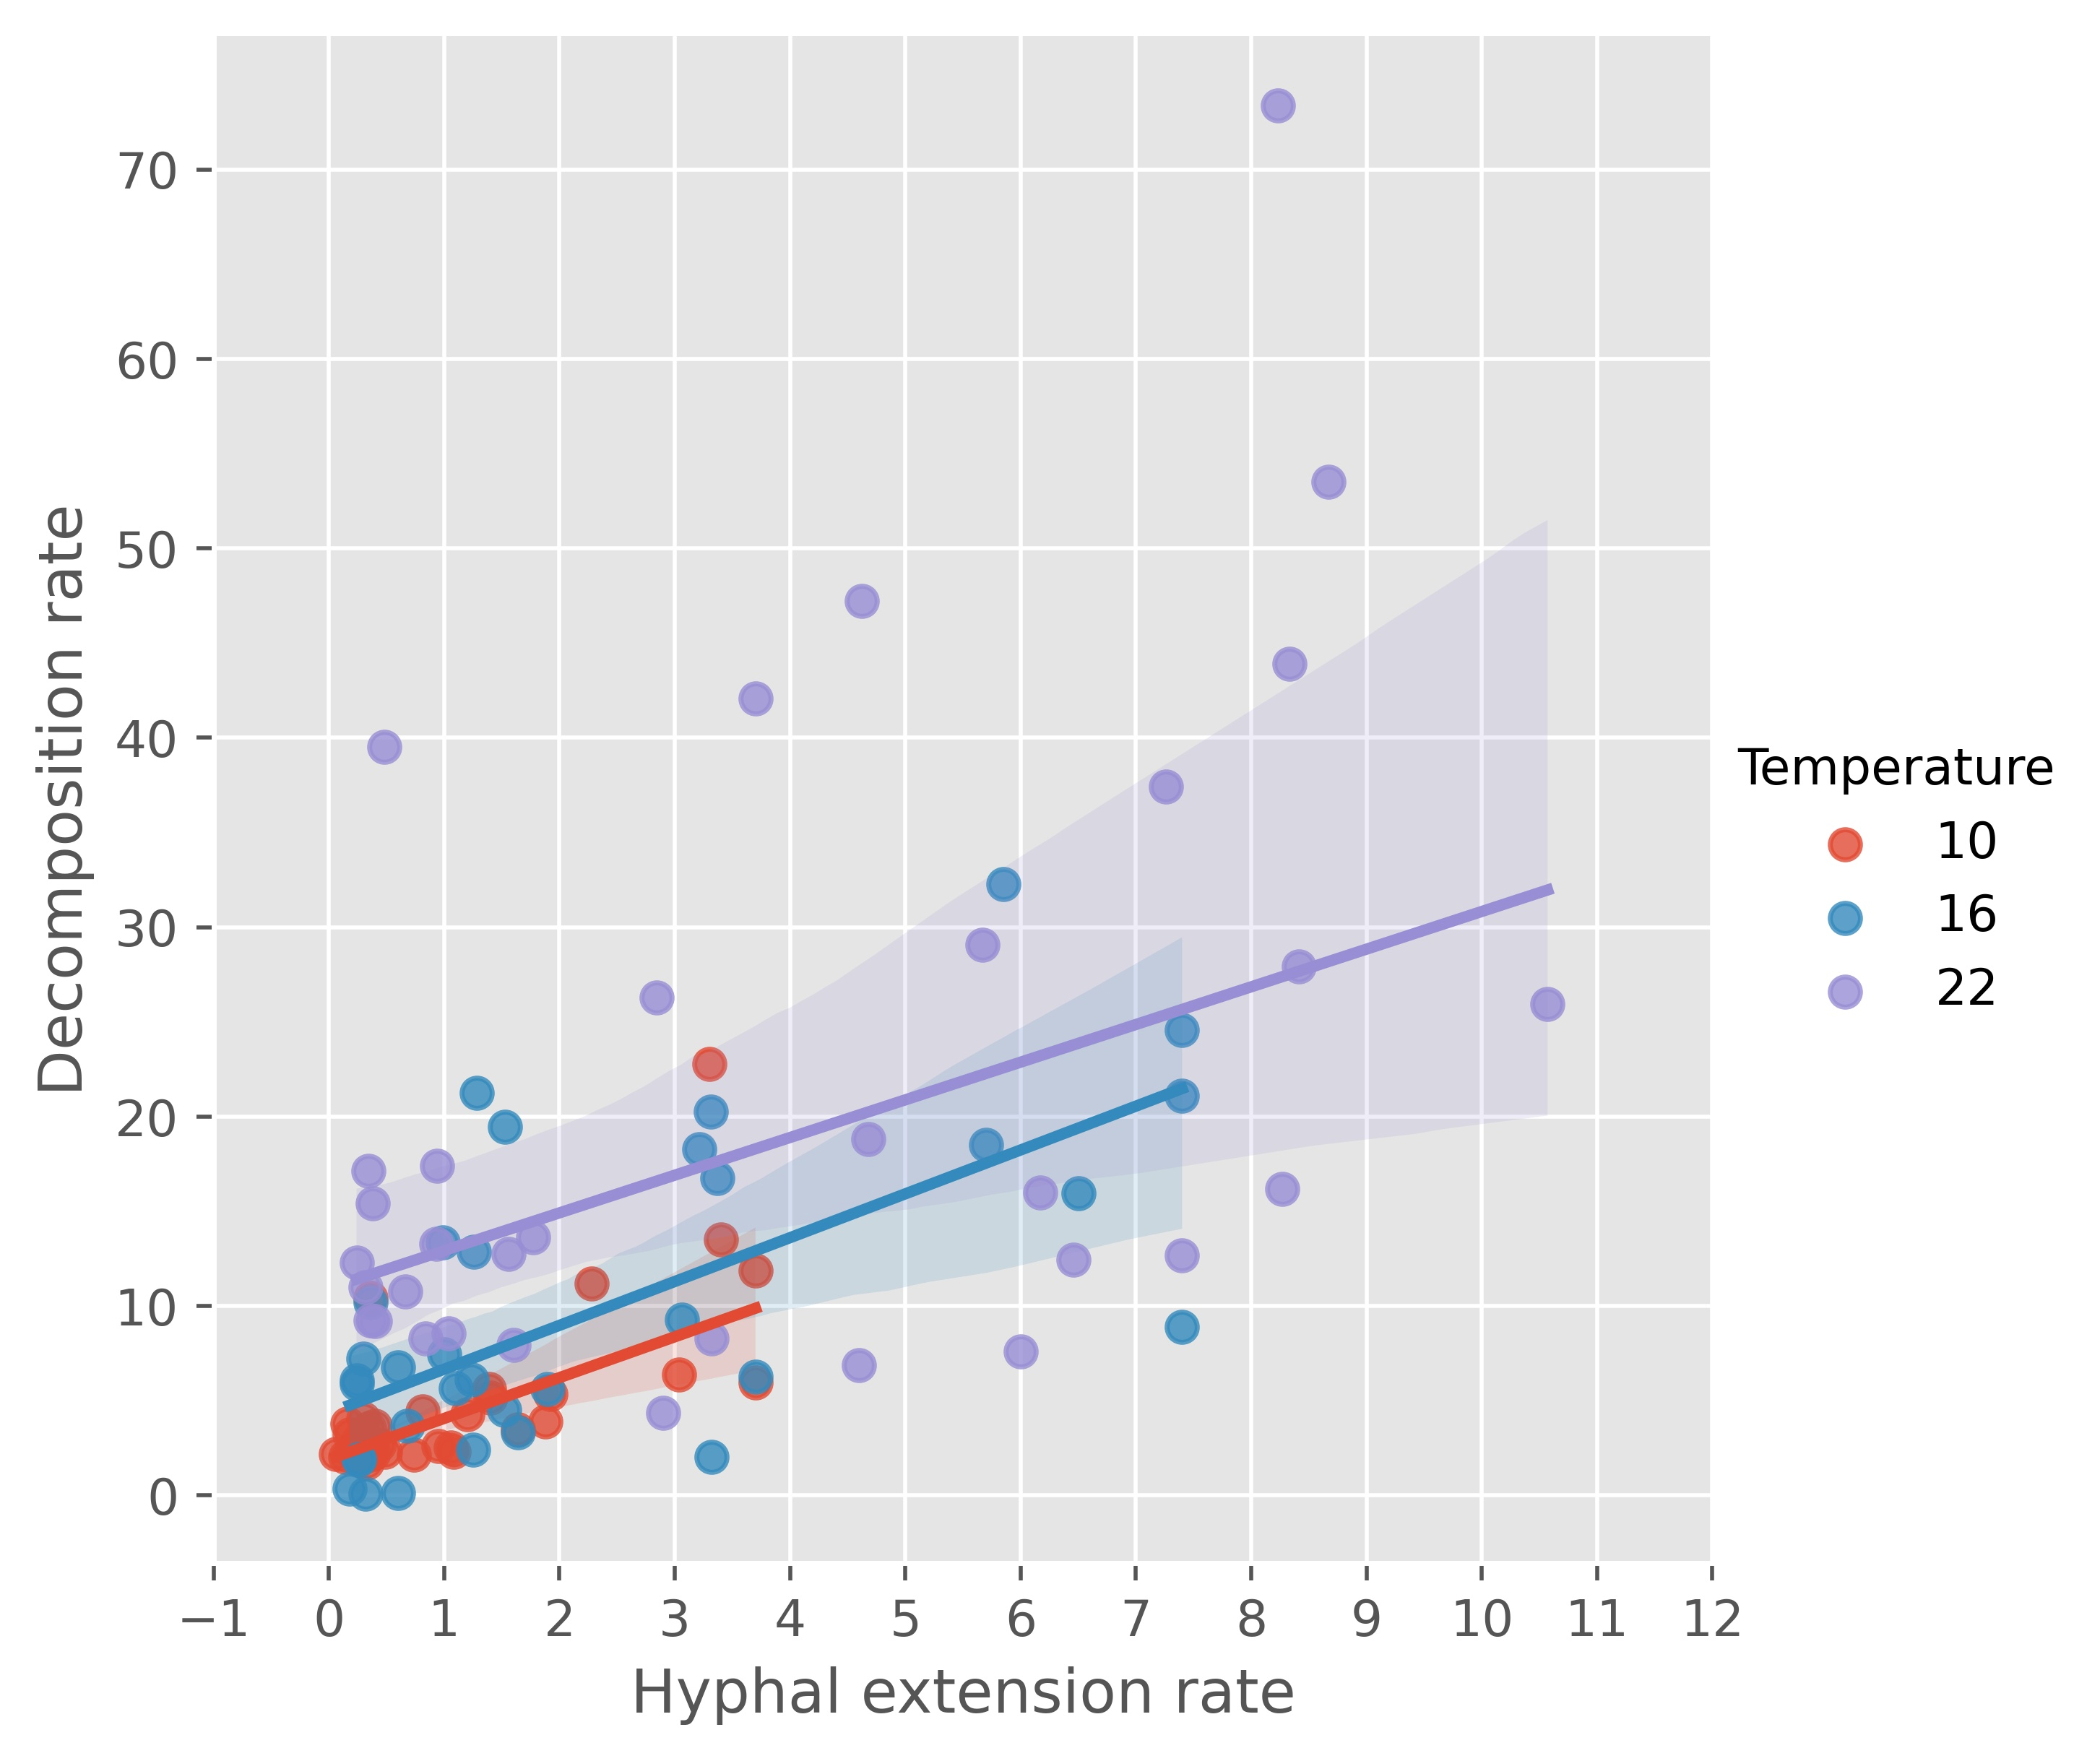
\includegraphics[scale=0.5]{./code/fig3.jpg}}
    \subfigure[]{
    \label{fig3b} 
    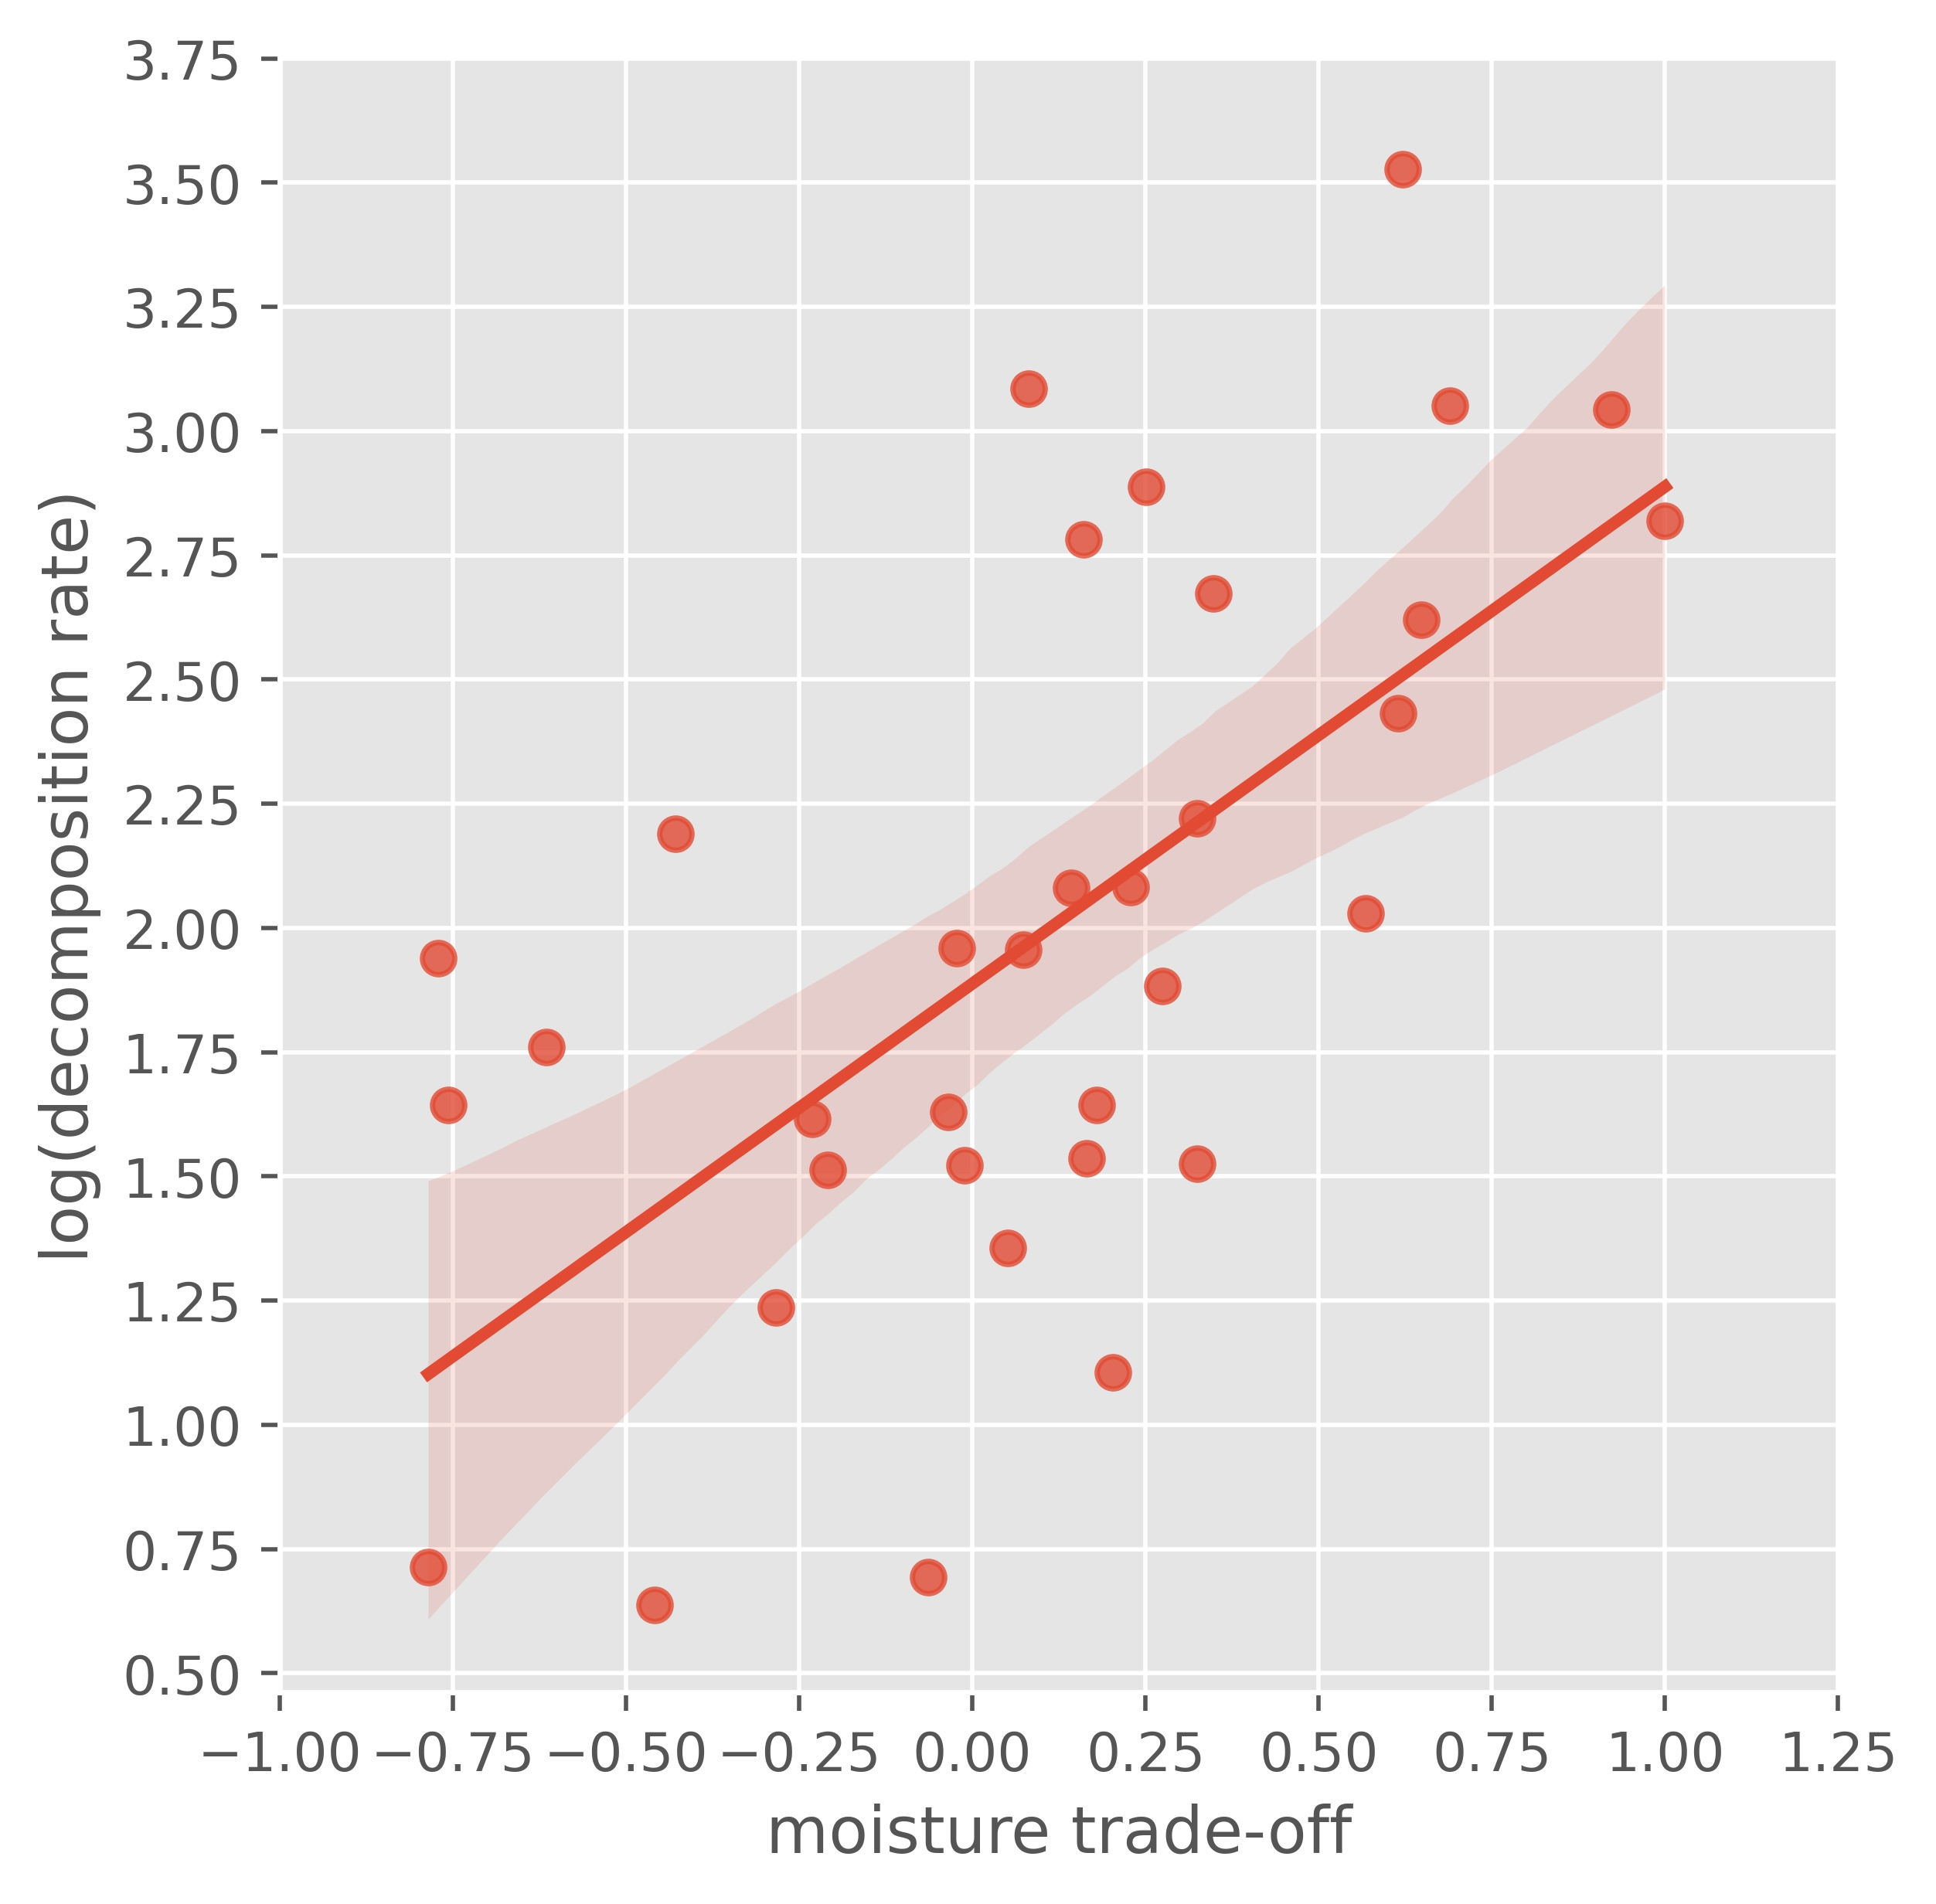
\includegraphics[scale=0.5]{./code/fig4.jpg}}
    \caption{Reproduce images from Papers}
    \label{fig3} 
\end{figure}

Therefore, assuming the decomposition rate as a constant value $Y$, the approximate relationship function between the hyphal extension rate and the decomposition rate and the approximate relationship function between the moisture trade-off and the decomposition rate can be selected as follows:
\begin{equation}\label{2.1}
    Y=a_{1}\ln{h}+b_{1}
\end{equation}
\begin{equation}\label{2.2}
    \ln{Y}=a_{2}m+b_{2}
\end{equation}

Where,

$h$ is the hyphal extension rate;

$m$ is moisture trade-off;

$a_{1}$ , $b_{1}$ , $a_{2}$ and $b_{2}$ are assumed coefficients.

After the correlation between the approximate relation function formula (\ref{2.1}) and the approximate relation function formula (\ref{2.2}), the relationship between the moisture trade-off and the hyphal extension rate can be obtained:
\begin{equation}\label{2.3}
    m=\frac{\ln{b_{1}}}{a_{1}}\ln{(a_{1}\ln{h})}-\frac{b_{2}}{a_{1}} 
\end{equation}

Then, the influences of the hyphal extension rate and moisture trade-off on decomposition rate are combined in a linear relationship, and the results are as follows:
\begin{equation}\label{2.4}
    y=am+bh+c 
\end{equation}

According to the relationship between moisture trade-off and the hyphal extension rate described in Equation (\ref{2.3}), the effects of the two factors can be combined, and then the equation (\ref{2.4}) can be converted into the expression of the decomposition rate about the hyphal extension rate:
\begin{equation}\label{}
    y=a\frac{\ln{b_{1}}}{a_{1}}\ln{(a_{1}\ln{h})}+bh+c-a\frac{b_{2}}{a_{1}} 
\end{equation}

Then simplify the above equation, and get
\begin{equation}\label{}
    y=r_{1}\ln{(r_{0}\ln{h})}+r_{2}h+r_{3}
\end{equation}

Where $r_{0},r_{1},r_{2},r_{3}$ are coefficients.

The real situation is complicated by the fact that there are many and different types of independent variables that affect the decomposition rate. In this model, linear equations are used for fitting. While simplifying the problem, the influence of various variables on the decomposition rate is also taken into consideration. And when using this model, the error of the result will decrease with the increase of data. Therefore, for the follow-up model research, our team chose to build the model with linear equations.

\subsubsection{Solution of Problem 2}

Using the above model, we can fit the relationship between decomposition rate and hyphal extension rate at different temperatures:
\begin{equation}\label{}
\left\{
\begin{array}{l}
    y=2.73x+1.855, when\ temperature = 10; (R^2=0.50)\\
    y=2.247x+4.799, when\ temperature = 16; (R^2=0.41) \\
    y=2.509x+11.48, when\ temperature = 22; (R^2=0.25) \\
\end{array}
\right.
\end{equation}
And the relationship between the decomposition rate and moisture trade-off is as follows:

\begin{equation}\label{}
    y=x+1.888; (R^2=0.40)
\end{equation}

Then, the effects of the hyphal extension rat and moisture trade-off on decomposition rate are combined with a linear relationship, and the relationship expression among the three can be obtained:
\begin{equation}\label{}
    y=0.37x_{1}+0.37x_{2}+2.07; (R^2=0.61)
\end{equation}

Where,

$x_{1}$ is the log(Hyphal extension rate)

$x_{2}$ is the moisture trade-off

$y$ is the log(decomposition rate)

The relation expression of the three is represented by Figure (\ref{4}):
\begin{figure}[H]
    \centering
    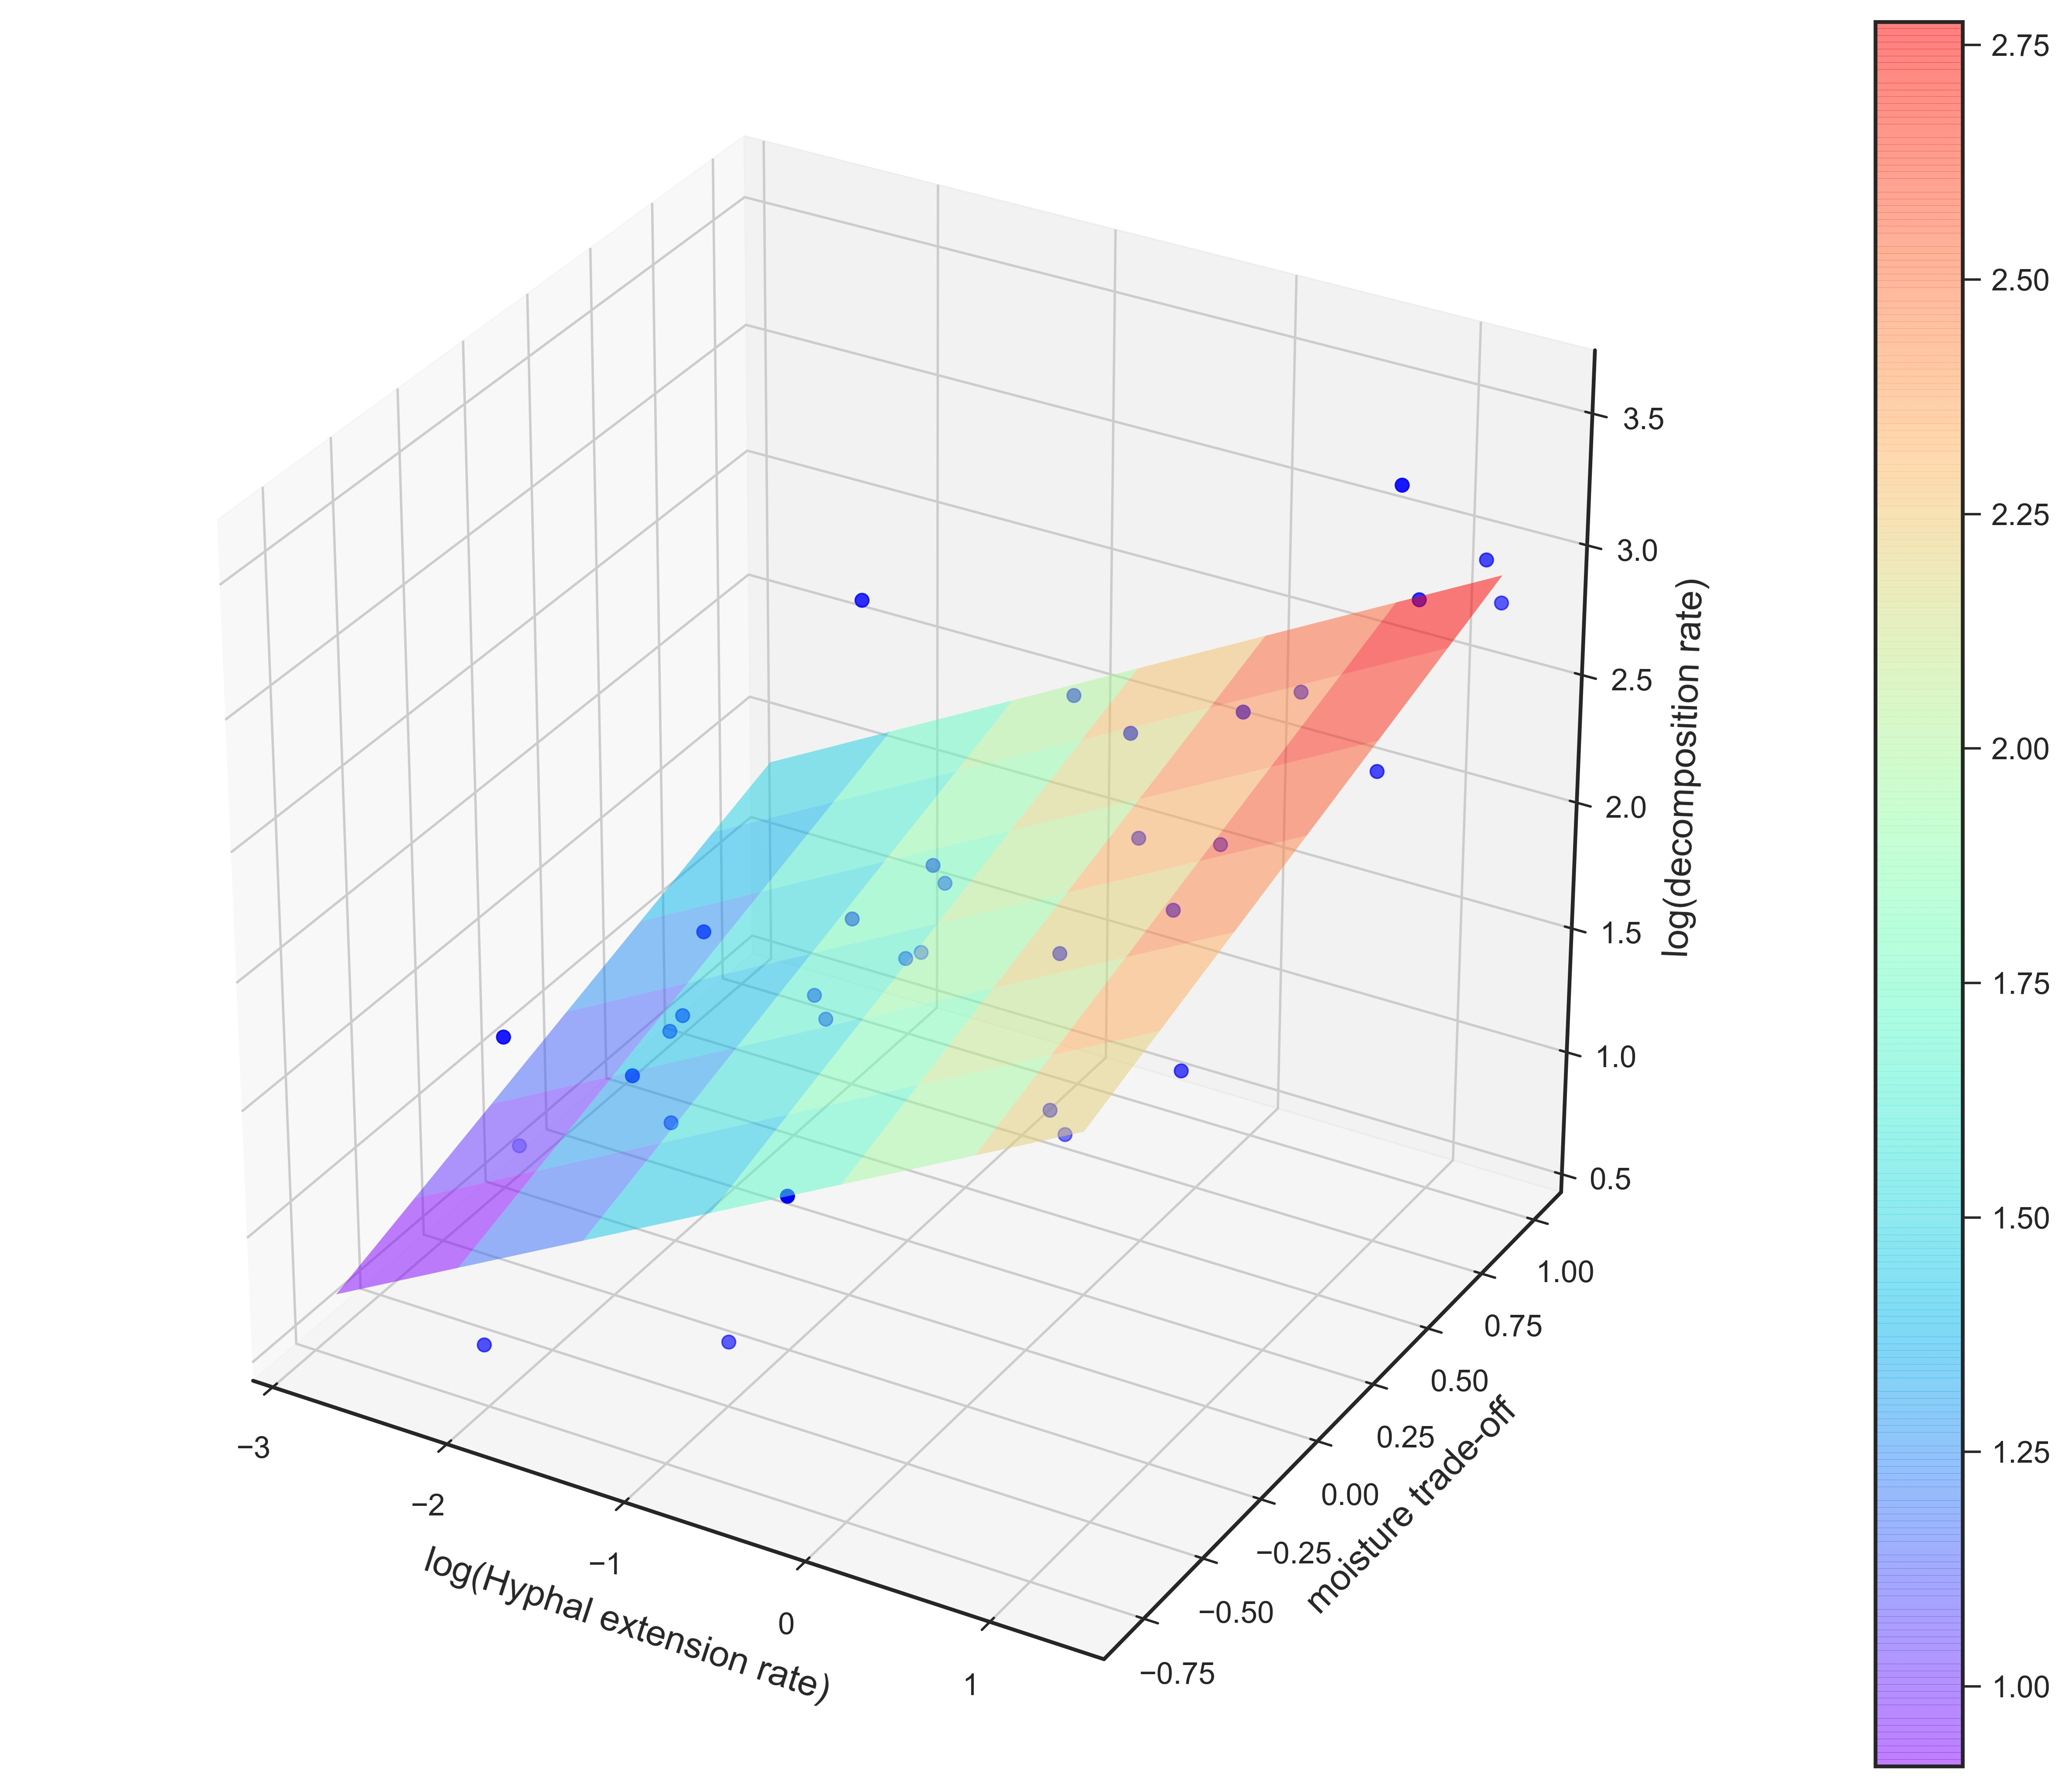
\includegraphics[width=0.8\textwidth]{./code/fig5.jpg}
    \caption{Combine hyphal extension rate and moisture trade-off on decomposition rate}\label{4}
\end{figure}

Through the fitting of the image of Decomposition rate -- Hyphal extension rate, we find that the fitting effect with "logarithmic relationship" is far less good than that with "linear relationship". Therefore, Equations (\ref{2.1}) and (\ref{2.3}) are improved to Equations (\ref{2.1*}) and (\ref{2.3*}).
\begin{equation}\label{2.1*}
    Y=a_{1}h+b_{1}
\end{equation}
\begin{equation}\label{2.3*}
    m=\frac{\ln{b_{1}}}{a_{1}}\ln{(a_{1}h)}-\frac{b_{2}}{a_{1}} 
\end{equation}

After combining Hyphal Extension Rate and Moisture Trade-Off, the following formula can be obtained:
\begin{equation}\label{2.5}
    y=r_{1}\ln(r_{0}h)+r_{2}h+r_{3}
\end{equation}

The results obtained by this method accord with the expected effect and the error is small.
    \subsection{Problem 3}
\subsubsection{Dynamic interaction model}

"Competition" refers to the struggle for existence between two or more individuals within or between species, whose demands more or less exceed the supply of common resources, thus exerting adverse effects on each other among these competing individuals. In this question, different types of fungi compete for space and resources to survive in the same environment, so the interaction between them is usually manifested as competition, that is, competition between different populations.Our model needs to address what types of community evolution occur between different types of fungi under the same initial environment.
\begin{itemize}
    \item [(1)] 
    \textbf{Logistic model and Lotka-Volterra model}
\end{itemize}

At the beginning, the two or more fungal populations do not compete with each other under the condition of adequate nutrient supply. However, when the number of fungi more suitable for the environment is much larger than that of the weaker species, the weaker species will lack nutrients and may die. That is, when different types of fungi compete for the same food source and space, the common outcome is that the less competitive ones go extinct and the more competitive ones reach the maximum capacity that the environment allows. The population competition model can be used to describe the process of competition between different types of fungi and to analyze the conditions that produce the evolutionary outcomes of various communities.

When fungus 1 and fungus 2 are present, an increase in the number of one inhibits the growth of the other, given limited space and resources. Several parameters are used to represent the rules\upcite{jiang2} that the two fungi obey in the process of competition as follows:
\begin{equation}\label{3.1}
    \left\{
    \begin{array}{l}
        \frac{dN_{1}}{dt}=r_{1}N_{1}(1-\frac{N_{1}}{k_{1}}-\alpha \frac{N_{2}}{k_{1}}) \\
        \frac{dN_{2}}{dt}=r_{2}N_{2}(1-\frac{N_{2}}{k_{2}}-\beta \frac{N_{1}}{k_{2}}) \\
    \end{array}
    \right.
    \end{equation}

Where,

$N_{1}$ and $N_{2}$ are the size (expressed in number) of the two fungi;

$k_{1}$ and $k_{2}$ are the maximum environmental tolerance of the two fungi;

$r_{1}$ and $r_{2}$ are the growth rate of the two fungi;

$\alpha$ is the coefficient of competition of 1 to 2;

$\beta$ is the coefficient of competition of 2 to 1.

The coefficients of competition introduced here- $\alpha$ and $\beta$ represent the amount of one fungus that can be supported by the space and resources occupied by another fungus. Therefore, the inhibition relationship between fungi 1 and 2 can be reflected by the relationship between $k_{1}$ and $k_{2}$ . Through analysis, the inhibition relationship between the two fungi can be obtained as follows:

When $k_{2} > \frac{k_{1}}{\alpha}$, Fungus 2 can inhibit Fungus 1;

When $k_{2} < \frac{k_{1}}{\alpha}$, Fungus 2 can’t inhibit Fungus 1;

When $k_{1} > \frac{k_{2}}{\beta}$, Fungus 1 can inhibit Fungus 2;

When $k_{1} < \frac{k_{2}}{\beta}$, Fungus 1 can’t inhibit Fungus 2.
\begin{itemize}
    \item [(2)] 
    \textbf{Model singularity and type analysis}
\end{itemize}

In the process of competition, when both Equations in (\ref{3.1}) are zero, both Fungi 1 and Fungi 2 stop growing, and the system is relatively stable. It's easy to know that its singularity in the first quadrant is $E_{1}(0,0),E_{2}(k_{1},0),E_{3}(0,k_{2})$ and $E_{4}(k_{1}-\alpha k_{2},k_{2}-\beta k_{1})$.

\begin{itemize}
    \item [a)] 
    The linear equations corresponding to the singularity $E_{1}(0,0)$ are
    \begin{equation}\label{}
        \left\{
        \begin{array}{l}
            \frac{dN_{1}}{dt}=r_{1}N_{1} \\
            \frac{dN_{2}}{dt}=r_{2}N_{2} \\
        \end{array}
        \right.
        \end{equation}
    
    The coefficient matrix characteristic equation of the linear equations is $(\lambda-r_{1})(\lambda-r_{2})=0$, so $E_{1}(0,0)$ is the unstable point.

    \item [b)]
    Transform the singularity $E_{2}(k_{1},0)$ as follows:
    \begin{equation}\label{}
        \widetilde{N_{1}}=N_{1}-k_{1},\widetilde{N_{2}}=N_{2}
    \end{equation}

    The corresponding linear system of equations are:
    \begin{equation}\label{}
        \left\{
        \begin{array}{l}
            \frac{d\widetilde{N_{1}}}{dt}=r_{1}(\widetilde{N_{1}}+k_{1})(\frac{-\alpha\widetilde{N_{2}}-\widetilde{N_{1}}}{k_{1}}) \\
            \frac{d\widetilde{N_{2}}}{dt}=r_{2}\widetilde{N_{2}}(\frac{k_{2}-\widetilde{N_{2}}-\beta\widetilde{N_{1}}}{k_{2}})
        \end{array}
        \right.
        \end{equation}

    The characteristic equation of the corresponding coefficient matrix is $(\lambda+r_{1})(\lambda-r_{2})=0$, so $E_{2}(k_{1},0)$ is the saddle point.

    \item [c)]
    Similarly, the coefficient matrix characteristic equation of the linear system corresponding to $E_{3}(0,k_{2})$ can be obtained as $[\lambda-(r_{1}-\frac{r_{1}\alpha k_{2}}{k_{1}})](\lambda+r_{2})=0$

    So when $(k_{1}-\alpha k_{2})>0$, $E_{3}(0,k_{2})$ is the saddle point; when $k_{1}-\alpha k_{2}<0$, $E_{3}(0,k_{2})$ is the stable node.

    \item [d)]
    Transform the singularity $E_{4}(k_{1}-\alpha k_{2},k_{2}-\beta k_{1})$ as follows:
    \begin{equation}\label{}
        \widetilde{N_{1}}=N_{1}-(k_{1}-\alpha k_{2}),\widetilde{N_{2}}=N_{2}-(k_{2}-\beta k_{1})
    \end{equation}

    The corresponding linear system of equations are:
    \begin{equation}\label{}
        \left\{
        \begin{array}{l}
            \frac{d\widetilde{N_{1}}}{dt}=\frac{r_{1}}{k_{1}}[\widetilde{N_{1}}+(k_{1}-\alpha k_{2})](-\alpha\widetilde{N_{2}}-\widetilde{N_{1}}) \\
            \frac{d\widetilde{N_{2}}}{dt}=\frac{r_{2}}{k_{2}}[\widetilde{N_{2}}+(k_{2}-\beta k_{1})](-\beta\widetilde{N_{1}}-\widetilde{N_{2}}) \\
        \end{array}
        \right.
        \end{equation}
    
    The corresponding characteristic equation is $[\lambda+\frac{r_{1}(k_{1}-\alpha k_{2})}{k_{1}}][\lambda+\frac{r_{2}(k_{2}-\beta k_{1})}{k_{2}}]=0$, so $E_{4}(k_{1}-\alpha k_{2},k_{2}-\beta k_{1})$ is the stable point.

\end{itemize}

\begin{itemize}
    \item [(3)] 
    \textbf{Stability analysis}
\end{itemize}

According to the first approximation theory\upcite{jiang3}, it can be known that $E_{1}(0,0)$ and $E_{2}(k_{1},0)$ are unstable solutions, and $E_{4}(k_{1}-\alpha k_{2},k_{2}-\beta k_{1})$ is asymptotically stable solution. As for the property of $E_{3}(0,k_{2})$, we need to discuss it in three cases:

When $k_{1}-\alpha k_{2}>0$, $E_{3}(0,k_{2})$ is unstable;

when $k_{1}-\alpha k_{2}<0$, $E_{3}(0,k_{2})$ is asymptotically stable;

when $k_{1}-\alpha k_{2}=0$, the Liapunov function is as follows:
    $$V_{(N_{1},N_{2})}=\frac{k_{1}}{r_{1}}N_{1}+\frac{k_{2}\alpha^2}{2r_{2}}(N_{2}-k_{2})^2>0 $$

Then the following expression can be obtained:
    \begin{equation}\label{}
    \begin{split}
    \frac{dv}{dt}&=\frac{dv}{dN_{1}}\frac{dN_{1}}{dt}+\frac{dv}{dN_{2}}\frac{dN_{2}}{dt} \\
    &=-[N_{1}+\frac{\alpha}{2}(N_{2}-k_{2})]^2-\frac{\alpha^2}{4}(4N_{2}-1)(N_{2}-k_{2})^2\\
    &<0 \\
    \end{split}
    \end{equation}

According to Liapunov's fundamental theorem, the corresponding solution to $E_{3}(0,k_{2})$ is asymptotically stable.

\begin{itemize}
    \item [(4)] 
    \textbf{The balance of the two fungi}
\end{itemize}

According to the above stability analysis, four results as shown in the following table can be seen under different inhibition relationships.
    \begin{longtable}{|p{.3\textwidth}|p{.33\textwidth}|p{.33\textwidth}|}
        \caption{Different inhibition relationships} \\
        \hline
         & Fungus 1 inhibits 2 & Fungus 1 disinhibits 2 \\ 
         & $(k_{1} > \frac{k_{2}}{\beta})$ & $(k_{1} < \frac{k_{2}}{\beta})$ \\ \hline

         Fungus 2 inhibits 1 & Either Fungus 1 or 2 survives & Fungus 2 survives \\  

        $(k_{2} > \frac{k_{1}}{\alpha})$ & (\uppercase\expandafter{\romannumeral1}) & (\uppercase\expandafter{\romannumeral2})\\ \hline

        Fungus 2 disinhibits 1 & Fungus 1 survives & A balance of Fungus 1 and 2 \\

        $(k_{2} < \frac{k_{1}}{\alpha})$ & (\uppercase\expandafter{\romannumeral3}) & (\uppercase\expandafter{\romannumeral4})\\ \hline
        
        \end{longtable}

The above four results are represented by balance lines. It can be find that under the situation (\uppercase\expandafter{\romannumeral3}) and (\uppercase\expandafter{\romannumeral2}) balance lines of fungus 1 and fungus 2 have no intersection, so the system can't achieve balance and one side of the two will be eliminated;Under the situation (\uppercase\expandafter{\romannumeral1}) although there is a balance, but tiny fluctuations will lead to the system state deviation from equilibrium; situation (\uppercase\expandafter{\romannumeral4}) is a stable equilibrium, when the time is long enough, any initial state is gradually reaching balance, make the system to reach equilibrium.
    \begin{figure}[H]
        \centering
        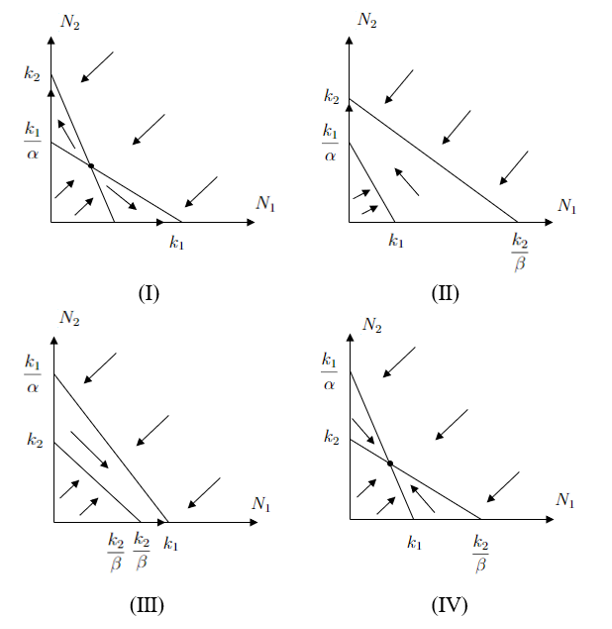
\includegraphics[width=0.55\textwidth]{./code/fig6.png}
        \caption{Four results represented by balance lines}\label{fig6}
    \end{figure}
    
By using the curve representation, we can more intuitively observe the interaction between the two fungi and the different evolution of the system under different inhibition relations.
    \begin{figure}[H]
        \centering
        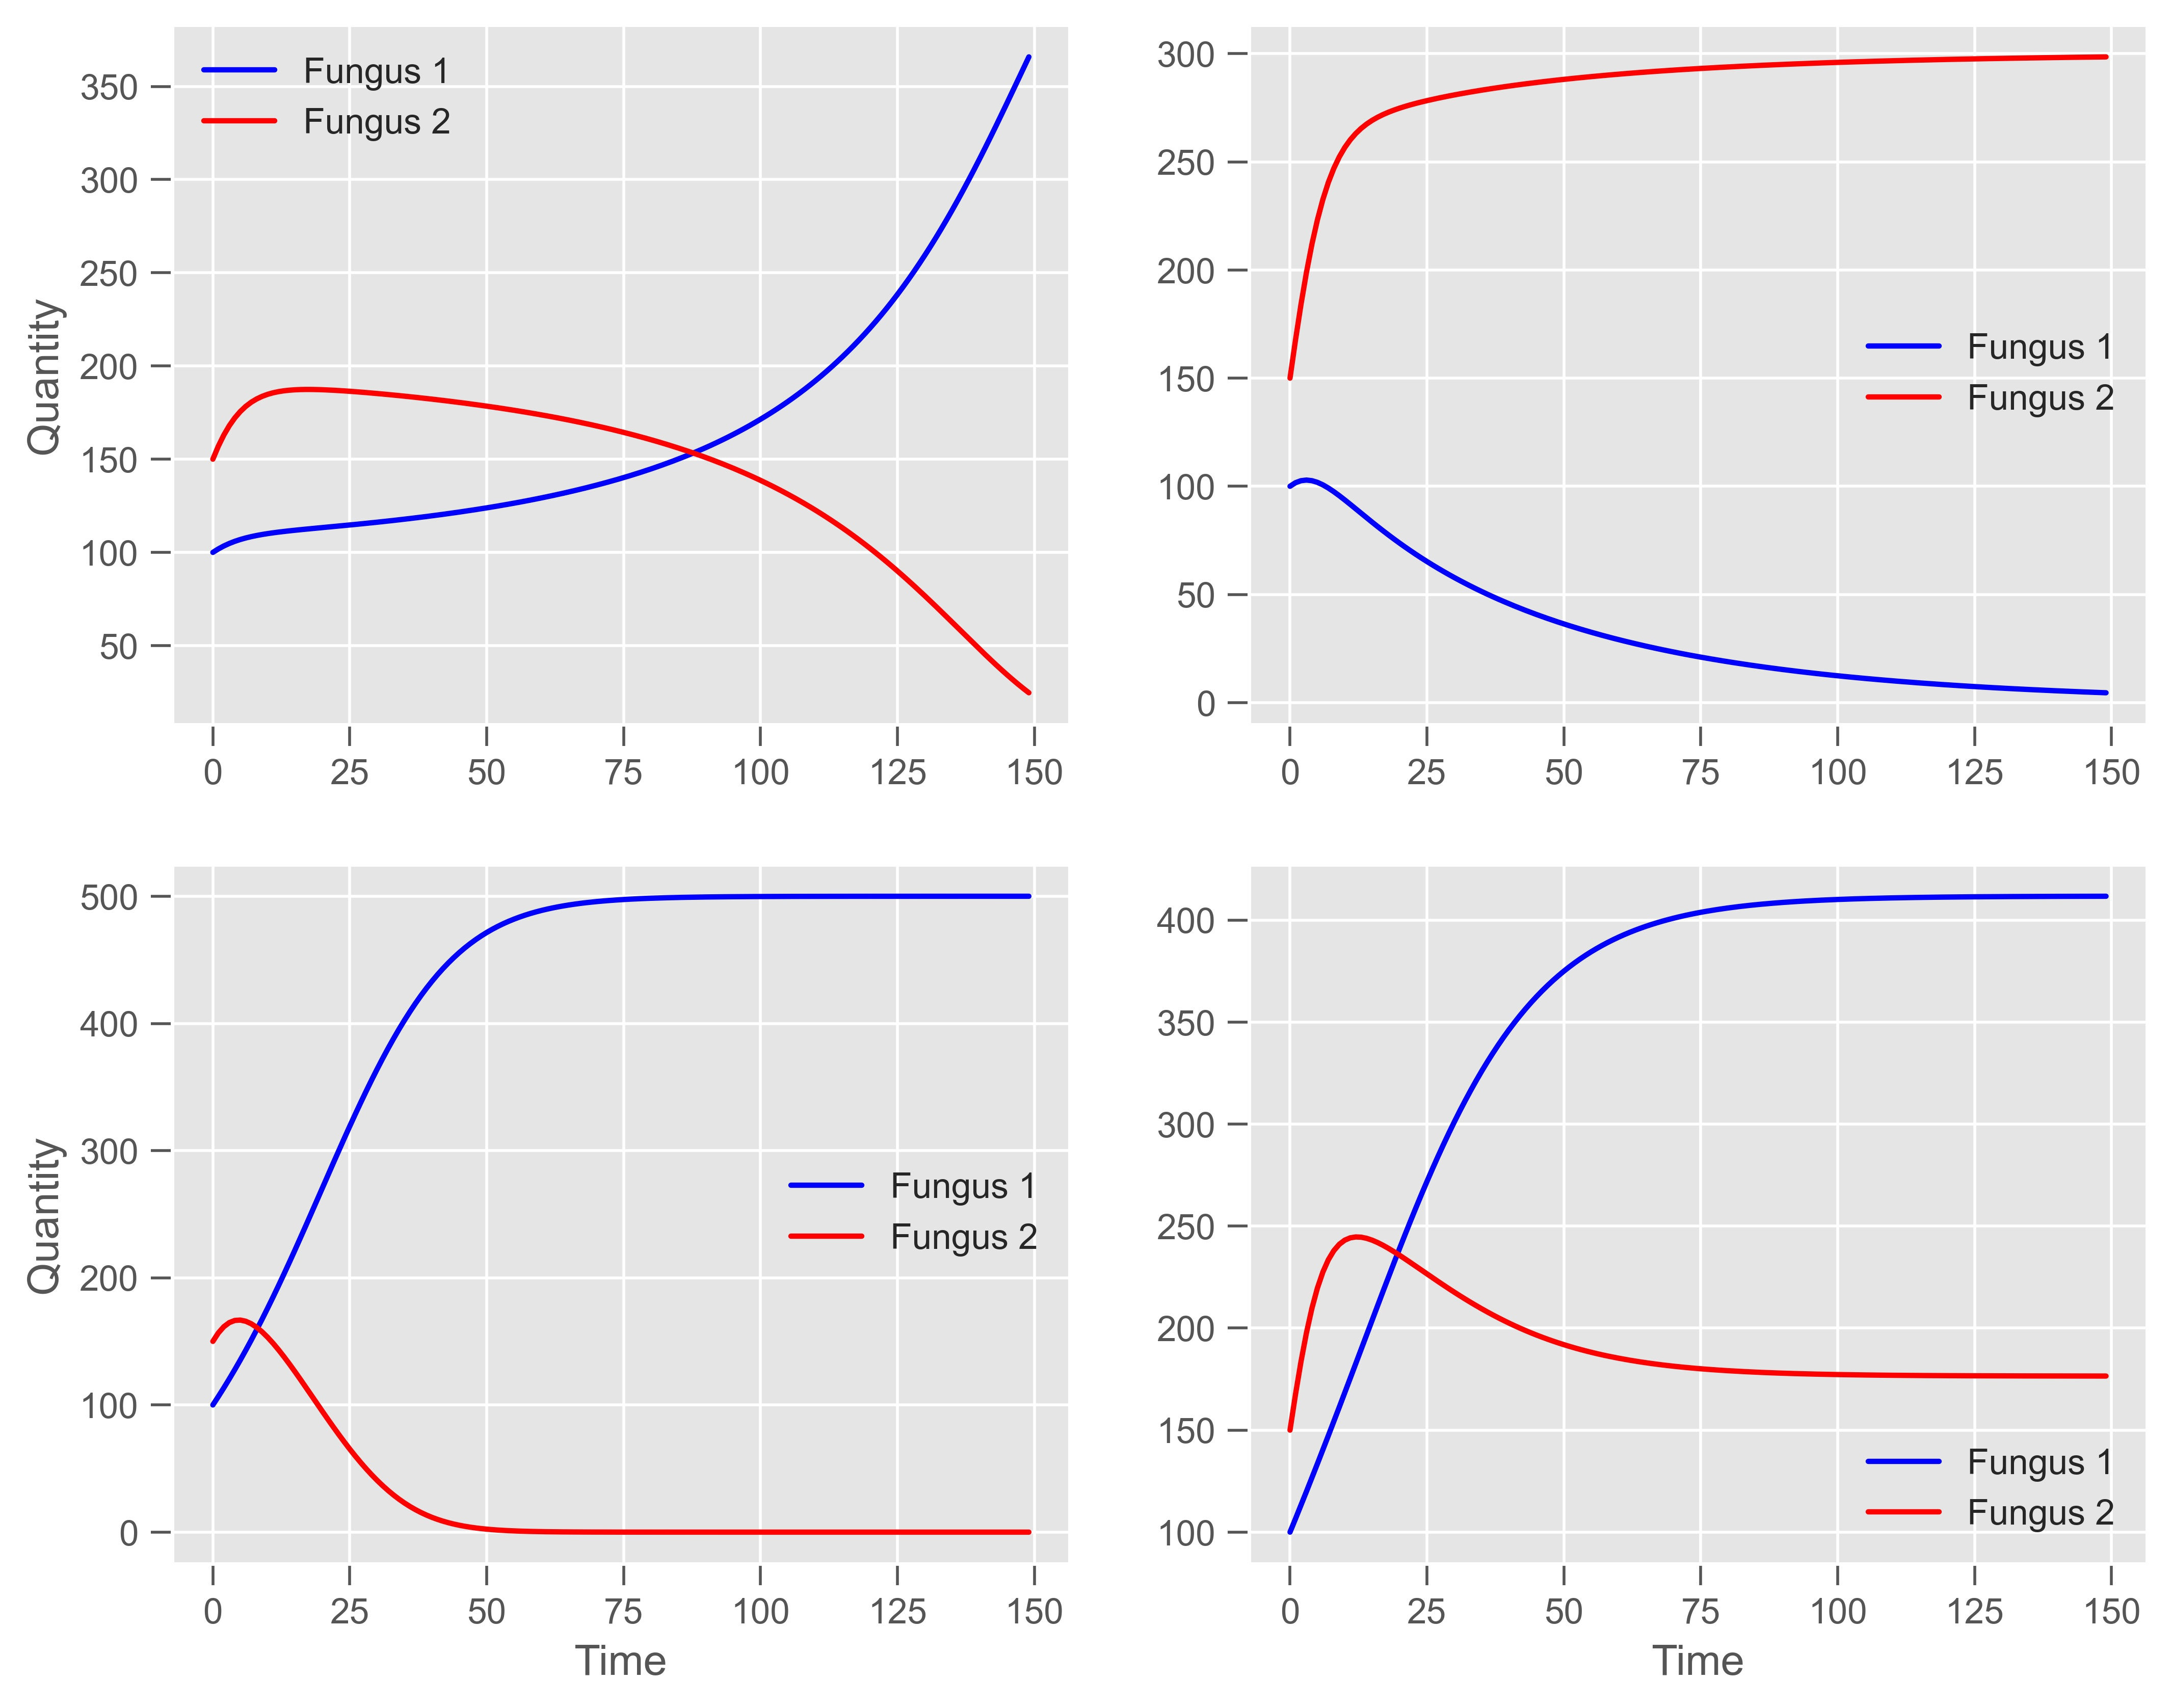
\includegraphics[width=0.6\textwidth]{./code/fig7.jpg}
        \caption{Four results represented by curves}\label{fig7}
    \end{figure}

\subsubsection{Solution of Problem 3}

When the atmospheric environment changes, it will cause changes in the correlation coefficient $k_{1},k_{2},r_{1},r_{2},\alpha,\beta$, which will affect the model and the long-term and short-term trends, resulting in changes in the four situations shown in Figure (\ref{fig6}). Combined with Table (2), it can be seen that situation (\uppercase\expandafter{\romannumeral1}) is most sensitive to the rapid fluctuation of the environment, and the rapid fluctuation determines the direction in which $N_{1},N_{2}$ moves from the equilibrium point and affects which one of Fungus 1 and Fungus 2 is eliminated in the end. That is to say, when $k_{2}>\frac{k_{1}}{\alpha}$ and $k_{1}>\frac{k_{2}}{\beta}$ , the equilibrium state reached is very sensitive to the fluctuation of the atmospheric environment. Situation (\uppercase\expandafter{\romannumeral1}) (\uppercase\expandafter{\romannumeral2})and (\uppercase\expandafter{\romannumeral3}) has a certain ability to adjust the change of $N_{1},N_{2}$. In the short term, it will be affected by the fluctuation, but with the passage of time, this influence will be gradually eliminated.

According to the above analysis, the system may have four results when the two types of fungi exist simultaneously. When there is no inhibition between the two fungi, they will eventually reach a stable coexistence state, and the stable point is $E_{4}(k_{1}-\alpha k_{2},k_{2}-\beta k_{1})$ . When one partner is inhibiting the other, eventually the inhibiting partner will gain an advantage and the other partner will be eliminated. When both sides have an inhibiting effect on the other, the initial condition determines the final winner.

    \subsection{Problem 4}
\subsubsection{Species and environment prediction model}

On the basis of Problem 3, another expression of Lotka-Volterra model is used as follows:
\begin{equation}\label{4.1}
    \left\{
    \begin{array}{l}
        \frac{dx_{1}(t)}{dt}=x_{1}(t)[r_{10}-a_{11}x_{1}(t)-a_{12}x_{2}(t)] \\
        \frac{dx_{2}(t)}{dt}=x_{2}(t)[r_{20}-a_{21}x_{1}(t)-a_{22}x_{2}(t)]  \\
        x_{i}(t)>0, r_{i0}>0, a_{ij}>0,(i=1,2;j=1,2).
    \end{array}
    \right.
    \end{equation}

Where,

$x_{1}(t)$ and $x_{2}(t)$ are the scale of fungi 1 and 2 at time $t$ (described by number);

$r_{i}(0)$ is the growth rate within the population;

$a_{ij}$ is the competition coefficient within the population (when $i=j$) or the competition coefficient between the populations (when $i\neq j$).

Let $C_{0}(t)$ represent the amount of external factors influencing individuals at time $t$, and $C_{c}(t)$ represent the amount of external factors influencing the environment at time $t$. Assuming that the fungal population does not migrate and is homogeneous and introduces random disturbance, then:
\begin{equation}\label{}
    r_{i0} \to r_{i0} + \sigma_{i}^2 dB_{i}(t)
\end{equation}

Where,

$dB_{i}(t)$ is the interference of external variables;

$\sigma_{i}^2$ is Brown's exercise intensity.

The following stochastic population dynamic system is introduced into Equation (\ref{4.1}):
\begin{equation}\label{4.2}
    \left\{
    \begin{array}{l}
        dx_{1}(t)=x_{1}(t)[r_{10}-r_{11}C_{0}(t)-a_{11}x_{1}(t)]dt-x_{1}(t)a_{12}x_{2}(t)+\sigma_{1}x_{1}(t)dB_{1}(t) \\

        dx_{2}(t)=x_{2}(t)[r_{20}-r_{21}C_{0}(t)-a_{21}x_{1}(t)]dt-x_{2}(t)a_{22}x_{2}(t)+\sigma_{2}x_{2}(t)dB_{2}(t) \\
        x_{i}(t)>0,i=1,2
    \end{array}
    \right.
    \end{equation}

$r_{i1}$ is the influence intensity of external factors on the dynamical system.

Through transformation, we can get:
\begin{equation}\label{4.3}
    \left\{
    \begin{array}{l}
        \frac{dC_{0}(t)}{dt}=kC_{c}(t)-(g+m)C_{0}(t) \\
        \frac{dC_{c}(t)}{dt}=-hC_{c}(t)+u(t) \\
    \end{array}
    \right.
    \end{equation}

The initial values of the two influences are $C_{0}(0)=C_{c}(0)=0$

Where,

$k,g,m,h$ are all normal numbers;

$kC_{c}(t)-gC_{0}(t)$ is the amount of external influence absorbed by the population from the environment at time $t$;

$mC_{0}(t)$ is the self-digesting amount of the population to the external environment at time $t$;

$-hC_{c}(t)$ is the self-digesting amount of the primary environment to external factors at time $t$;

$u(t)$ is the input rate of external disturbance to the environment.

The dynamic disturbance population model composed of (\ref{4.2}) and (\ref{4.3}) is analyzed, and the relevant symbols are defined as follows:

\begin{multicols}{2}
    $R_{+}=[0,+\infty ]$

    $R_{+}^0={a|a>0,a\in R}$

    $x^*=\lim_{t \to +\infty}\sup x(t)$

    $x_{*}=\lim_{t \to +\infty}\inf x(t)$

    $[x(t)]=\int_{0}^tx(s)ds / t $

    $\Phi_{1}=a_{22}r_{11}-a_{12}r_{21}$

    $\Phi_{2}=a_{11}r_{21}+a_{21}r_{11}$

    $\Delta =a_{11}a_{22}+a_{21}a_{12}$

    $\delta =r_{11}(r_{20}-\frac{\sigma_{2}^2}{2})-r_{21}(r_{10}-\frac{\sigma_{1}^2}{2})$

    $\Delta_{1} =a_{22}(r_{10}-\frac{\sigma_{1}^2}{2})-a_{12}(r_{20}-\frac{\sigma_{2}^2}{2})$

    $\Delta_{2} =a_{11}(r_{20}-\frac{\sigma_{2}^2}{2})+a_{21}(r_{10}-\frac{\sigma_{1}^2}{2})$
\end{multicols}

Then we can get the following conclusion:

When $\lim_{t \to +\infty}x(t)=0$ a.s. fungal population $x (t)$ will extinct;

when $\lim_{t \to +\infty}[x(t)]=0$ a.s. fungal population $x(t)$ is not average persistent;

when $[x(t)]^*>0$ a.s. fungal population $x(t)$ is weakly average persistent;

when $[x(t)]_{*}\geqslant 0$ a.s. fungal population $x(t)$ is strongly average persistent.

According to the proof of Chen Shasha et al.\upcite{jiang4}, the above four results correspond to the following four dynamic interference situations:

\begin{itemize}
    \item [a)] 
    If $[C_{0}(t)]_{*}>\varphi (\psi )$, then $\lim_{t \to +\infty}x(t)=0$, that is, the population will be extinct.

    Where,
    \begin{equation}\label{}
        \varphi =
        \left\{
        \begin{array}{l}
            \frac{(r_{10}-\frac{\sigma_{1}^2}{2})}{r_{11}},\delta \leqslant 0 \\
            \frac{\Delta_{1}}{\Phi_{1}},\delta>0 \\
        \end{array}
        \right.
        \end{equation}
    
    \begin{equation}\label{}
        \psi  =
        \left\{
        \begin{array}{l}
            \frac{(r_{20}-\frac{\sigma_{2}^2}{2})}{r_{21}},\delta>0 \\
            \frac{\Delta_{2}}{\Phi_{2}},\delta\leqslant 0 \\
        \end{array}
        \right.
        \end{equation}

    \item [b)] 
    If $[C_{0}(t)]_{*}=\varphi ([C_{0}(t)]_{*}=\psi )$, then $\lim_{t \to +\infty}[x(t)]=0$, that is, the population is not average persistent;

    \item [c)] 
    If $[C_{0}(t)]_{*}<\varphi (\psi )$, then $[x(t)]^*>0$,that is, the population is weakly average persistent;

    \item [d)] 
    If $\lim_{t \to +\infty}[C_{0}(t)]$ is bounded and satisfies the following conditions:
    \begin{equation}\label{}
        \left\{
        \begin{array}{l}
            \Delta_{1}-\Phi_{1} \lim_{t \to +\infty}[C_{0}(t)]\geqslant 0 \\
            \Delta_{2}-\Phi_{2} \lim_{t \to +\infty}[C_{0}(t)]\geqslant 0 \\
        \end{array}
        \right.
        \end{equation}
    
    Then we can get
    \begin{equation}\label{}
        \lim_{t \to +\infty}[X_{1}(t)]=\frac{\Delta_{1}-\Phi_{1} \lim_{t \to +\infty}[C_{0}(t)]}{\Delta}\geqslant 0
    \end{equation}
    
    \begin{equation}\label{}
        \lim_{t \to +\infty}[X_{2}(t)]=\frac{\Delta_{2}-\Phi_{2} \lim_{t \to +\infty}[C_{0}(t)]}{\Delta}\geqslant 0
    \end{equation}

    that is, the population is strongly average persistent.
\end{itemize}

\subsubsection{Solution of Problem 4}

The comparative advantages and disadvantages of different types of fungi and different environments can be predicted through the above analysis.

Predictions about species: Fungi that have the ability to inhibit other fungi always have a comparative advantage, whether or not the fungal population is in an average persistent state. If no fungal population maintains a strongly average persistence, at least one fungal species will be extinct. Fungi that are inhibited by other fungi and are less competitive are at a relative disadvantage.

Predictions about different environments: In arid and semi-arid climate areas, the temperature difference between day and night is large and the humidity is low, so the fungi with strong resistance to temperature change and slow growth are in a comparative advantage. Temperatures in temperate climates vary seasonally, and ecosystems differ from season to season, so in this environment fungi that grow slowly can periodically gain an advantage. Rainforest climates are hot, rainy and relatively humid, so fungi that grow slowly and tolerate high temperatures and humidity are at an advantage.
\begin{figure}[H]
    \centering
    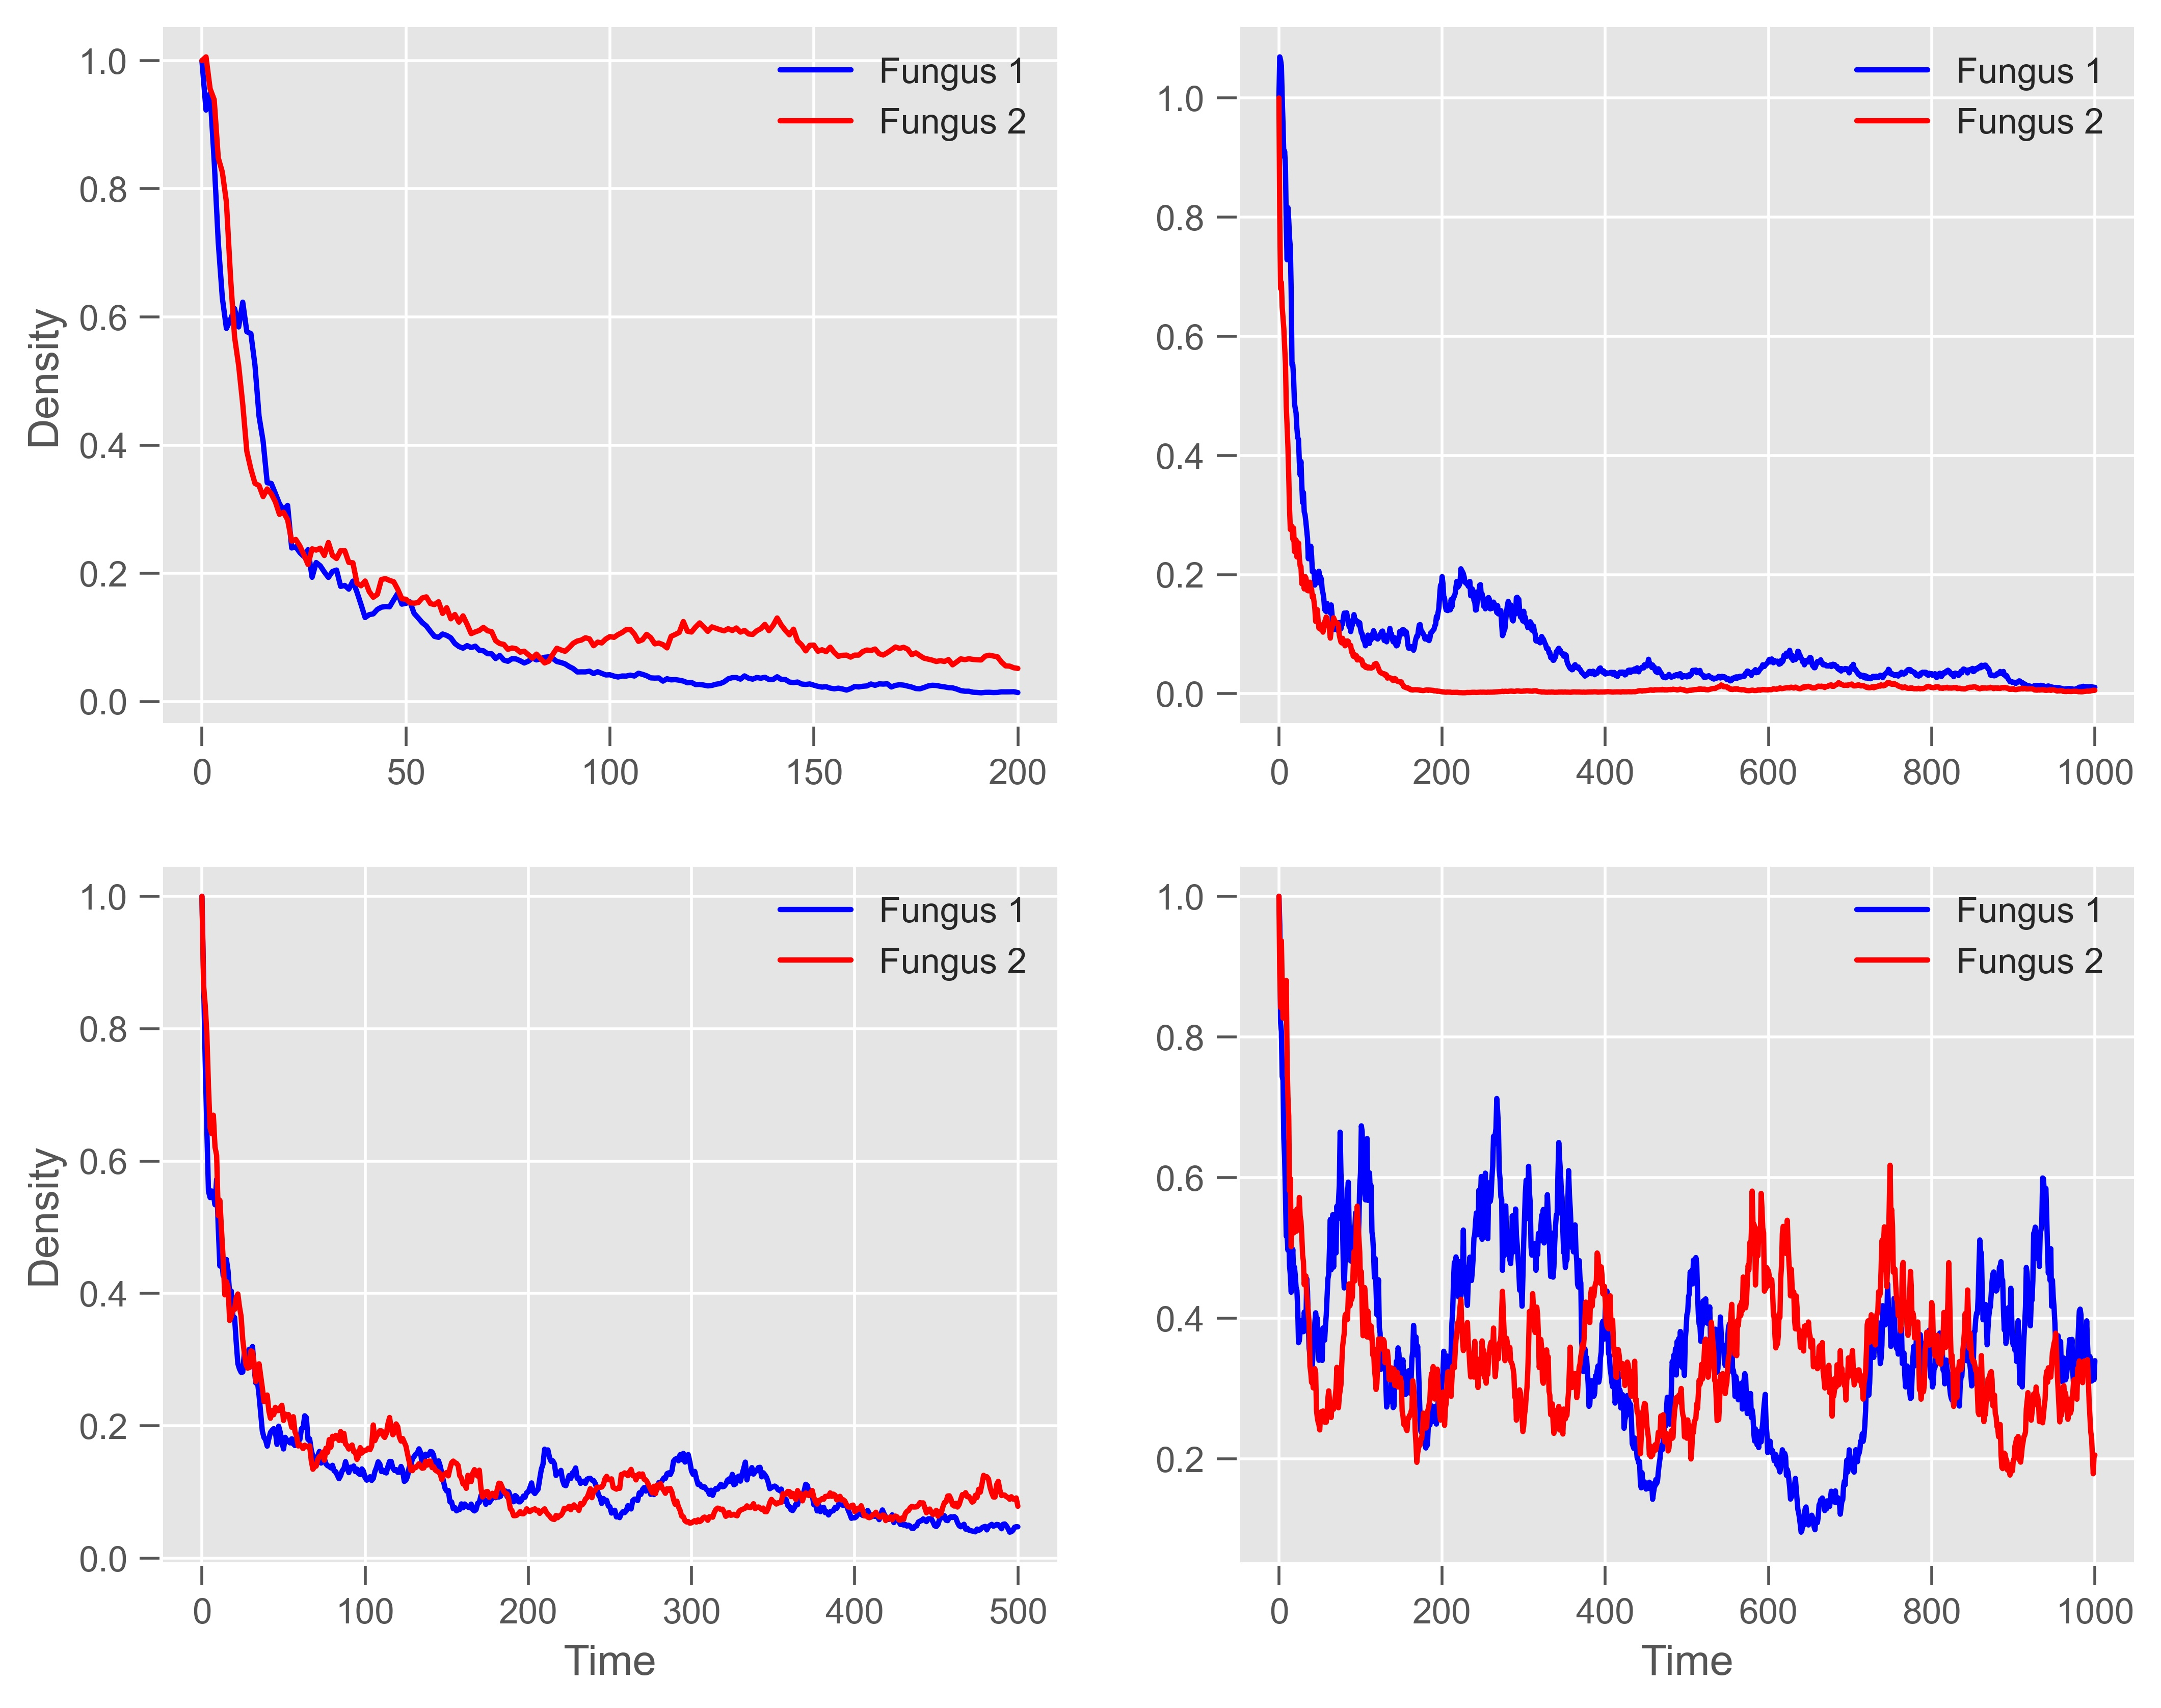
\includegraphics[width=0.6\textwidth]{./code/fig8.jpg}
    \caption{Dynamic change of Fungus 1 and 2}\label{fig8}
\end{figure}

For the first picture in Figure (\ref{fig8}):

$C_{0}(t)=0.2+0.01\sin t$

\begin{multicols}{5}
    $r_{10}=0.1$
    
    $r_{11}=0.5$
    
    $a_{11}=0.5$
    
    $a_{12}=0.5$
    
    $\sigma_{1}=0.2$

    $\sigma_{2}=0.2$
    
    $r_{20}=0.05$
    
    $r_{21}=0.6$
    
    $a_{21}=0.4$
    
    $a_{22}=0.5$

\end{multicols}

the second picture:

$C_{0}(t)=0.1+0.01\sin t$

\begin{multicols}{5}
    $r_{10}=0.1$
    
    $r_{11}=0.5$
    
    $a_{11}=0.5$
    
    $a_{12}=0.5$
    
    $\sigma_{1}=0.2$

    $\sigma_{2}=0.2$
    
    $r_{20}=0.05$
    
    $r_{21}=0.6$
    
    $a_{21}=0.4$
    
    $a_{22}=0.5$

\end{multicols}

the third picture:

$C_{0}(t)=0.001+0.001\sin t$

\begin{multicols}{5}
    $r_{10}=0.1$
    
    $r_{11}=0.5$
    
    $a_{11}=0.5$
    
    $a_{12}=0.5$
    
    $\sigma_{1}=0.2$

    $\sigma_{2}=0.2$
    
    $r_{20}=0.05$
    
    $r_{21}=0.6$
    
    $a_{21}=0.4$
    
    $a_{22}=0.5$

\end{multicols}

the fourth picture:

$C_{0}(t)=0.005+0.001\sin t$

\begin{multicols}{5}
    $r_{10}=0.4$
    
    $r_{11}=0.2$
    
    $a_{11}=0.5$
    
    $a_{12}=0.5$
    
    $\sigma_{1}=0.2$

    $\sigma_{2}=0.2$
    
    $r_{20}=0.3$
    
    $r_{21}=0.1$
    
    $a_{21}=0.4$
    
    $a_{22}=0.5$

\end{multicols}
    \subsection{Problem 5}
\subsubsection{Fungal diversity model}

The interaction between populations in an ecosystem is very complex, and its types can be roughly divided into three categories: first, neutral interaction, that is, there is no interaction between populations. In fact, living things are universally related to each other, and no interaction is relative. Secondly, positive interaction, which can be divided into three categories: partial symbiosis, original collaboration and mutualism. Third, negative interactions, including competition, predation, parasitism and bias, etc. In the third question, only the competition between different types of fungi is considered, and other interactions are not considered. In the real environment, the interaction between different types of fungi not only contains competition, but also may have positive interactions and other negative interactions. Therefore, this model needs to comprehensively consider the effects of various interactions on the decomposition rate.

Using fungal populations A, B and C as examples, in order to simulate the real environment in the coexistence of a variety of interaction, assuming that there is a positive interaction between fungus A and fungus B (such as the material produced by one party is good for the other and so on), and at the same time, there is a negative interaction (such as competition for survival resources and so on). Here, the relationship between A and B is simply called the competitive and cooperative relationship.

\begin{equation}\label{5.1}
    \left\{
    \begin{array}{l}
        \frac{dN_{1}}{dt}=N_{1}(a_{1}-b_{1}N_{1}-c_{1}N_{1}-d_{1}N_{2}) \\
        \frac{dN_{2}}{dt}=N_{2}(a_{2}-b_{2}N_{2}-c_{2}N_{3}-d_{2}N_{1}) \\
        \frac{dN_{3}}{dt}=N_{3}(a_{3}-b_{3}N_{3}+c_{3}N_{1}+d_{3}N_{2}) \\
    \end{array}
    \right.
    \end{equation}

Where, $N_{1},N_{2}$ and $N_{3}$ are the scales of fungus A, B and C, respectively.

The parameters satisfy the following equations:
\begin{equation}\label{}
    \left\{
    \begin{array}{l}
        a_{i}=\frac{\overline{a_{i}}[(-1)^n+1]}{2}+\frac{\overline{a_{i}}[(-1)^{n+1}+1]}{2},i=1,2,3 \\
        b_{i}=\frac{\overline{b_{i}}[(-1)^n+1]}{2}+\frac{\overline{b_{i}}[(-1)^{n+1}+1]}{2},i=1,2,3 \\
        c_{i}=\frac{\overline{c_{i}}[(-1)^n+1]}{2}+\frac{\overline{c_{i}}[(-1)^{n+1}+1]}{2},i=1,2,3 \\
        d_{i}=\{ \frac{\overline{d_{i}}[(-1)^n+1]}{2}+\frac{\overline{d_{i}}[(-1)^{n+1}+1]}{2}\}(-1)^n,i=1,2 \\
        d_{3}=\frac{\overline{d_{3}}[(-1)^n+1]}{2}+\frac{\overline{d_{3}}[(-1)^{n+1}+1]}{2} \\
    \end{array}
    \right.
    \end{equation}

Where,

$n \in N$, all the coefficients are positive.

$\overline{b_{i}}$ is the competition coefficient within the population of the ith species.

$\overline{a_{i}}$ is the growth rate within the population of the ith species.

$\overline{c_{i}}$ and $\overline{d_{i}}$ are the competition (or cooperation) coefficients of other species of fungi against the ith species of fungi.

Therefore, $R_{+}^3=\{h=(x,y,z)^T\in R^3 | h>0\}$ is a positive invariant set of system (\ref{5.1})\upcite{jiang5}. Combined with the model stability analysis in problem 3 and problem 4, it can be seen that if
\begin{equation}\label{}
    B=
    \begin{pmatrix}
        -b_{1} & -d_{1} & -c_{1} \\
        -d_{2} & -b_{2} & -c_{2} \\
        c_{3} & d_{3} & -b_{3}
    \end{pmatrix}
    \end{equation}

has a positive diagonal matrix, such that $WB+B^TW$ is positive definite and satisfies
\begin{equation}\label{}
    \left\{
    \begin{array}{l}
        |d_{1}+d_{2}| < \sqrt{b_{1}b_{2}} \\
        |c_{3}-c_{1}| < \sqrt{b_{1}b_{3}} \\
        |c_{2}-d_{3}| < \sqrt{b_{2}b_{3}} \\
    \end{array}
    \right.
    \end{equation}

then the positive equilibrium E is globally asymptotically stable. So the overall rate of decomposition is $y^*=\sum_{i = 1}^{3}y_{i}N_{i}$,where $y_{i}$ is the decomposition rate of the ith fungus.

\subsubsection{Solution of Problem 5}
Considering that the local environment may have varying degrees of variability, we can achieve different variability by setting different initial conditions for the system (\ref{5.1}).
\begin{figure}[H]
    \centering
    \subfigure[]{
    \label{fig9a} 
    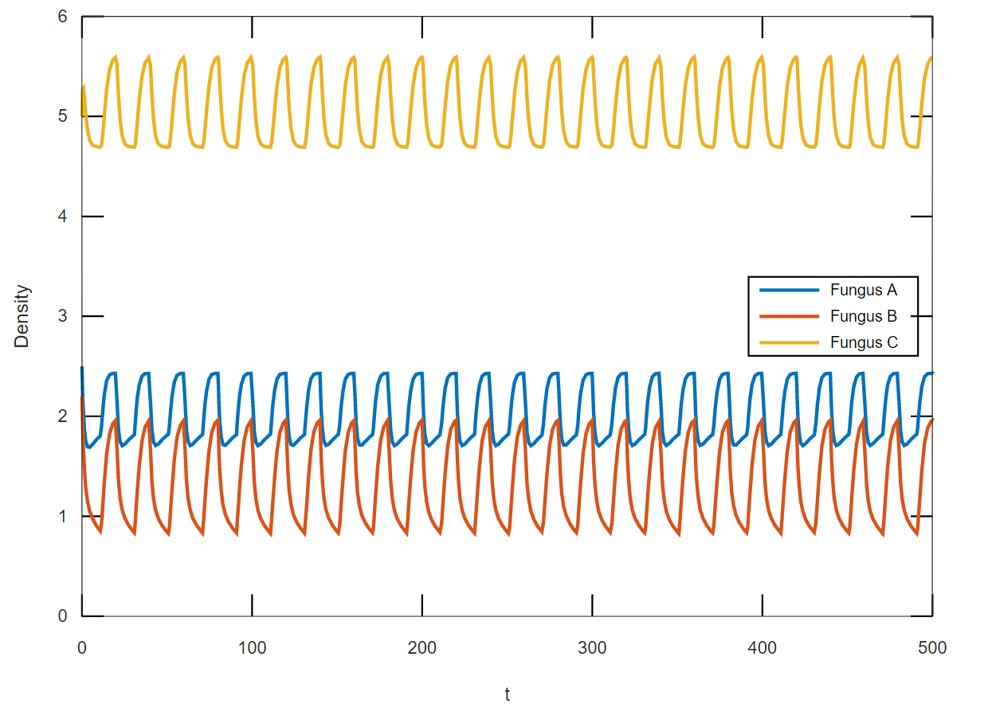
\includegraphics[scale=0.25]{./code/fig9.jpg}}
    \subfigure[]{
    \label{fig9b} 
    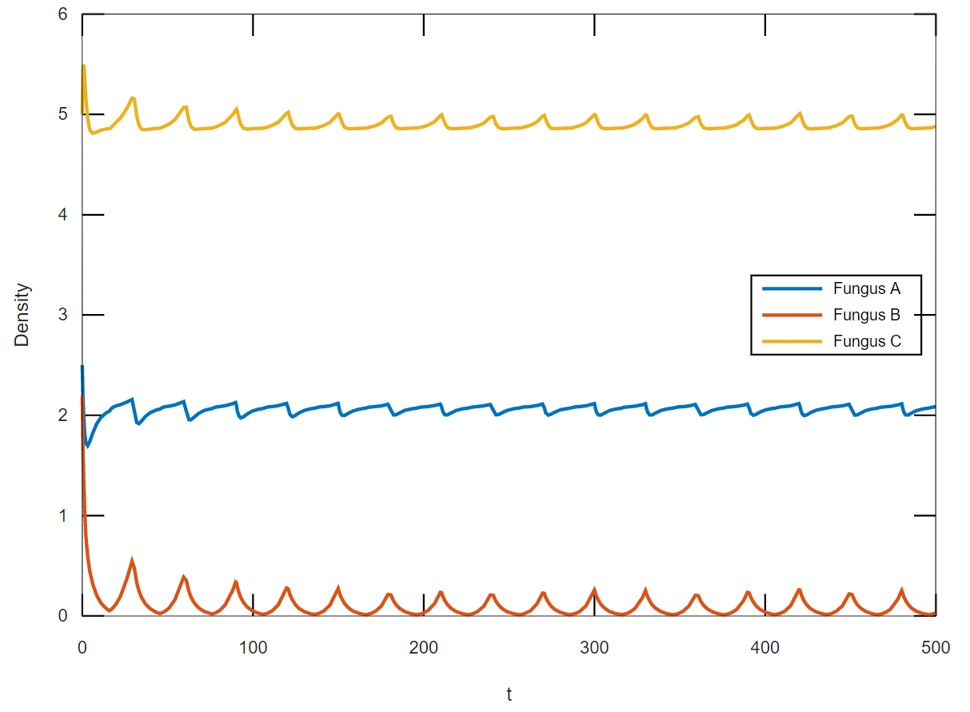
\includegraphics[scale=0.25]{./code/fig10.jpg}}
    \caption{Setting different initial conditions\upcite{zzwd}}
    \label{fig9} 
\end{figure}

For the figure (\ref{fig9a}):

\begin{multicols}{5}

    $N_{1}=2.50$

    $N_{2}=2.20$

    $N_{3}=5.00$

    $\overline{a_{1}}=1.00$

    $\overline{a_{2}}=1.00$

    $\overline{a_{3}}=0.80$

    $\overline{b_{1}}=0.20$

    $\overline{b_{2}}=0.15$

    $\overline{b_{3}}=0.25$

    $\overline{c_{1}}=0.12$

    $\overline{c_{2}}=0.16$

    $\overline{c_{3}}=0.15$

    $\overline{d_{1}}=0.08$

    $\overline{d_{2}}=0.08$

    $\overline{d_{3}}=0.12$ 

\end{multicols}

For the figure (\ref{fig9b}):

\begin{multicols}{5}

    $N_{1}=2.50$

    $N_{2}=2.20$

    $N_{3}=5.00$

    $\overline{a_{1}}=1.00$

    $\overline{a_{2}}=1.00$

    $\overline{a_{3}}=0.80$

    $\overline{b_{1}}=0.20$

    $\overline{b_{2}}=0.15$

    $\overline{b_{3}}=0.25$

    $\overline{c_{1}}=0.12$

    $\overline{c_{2}}=0.2$

    $\overline{c_{3}}=0.2$

    $\overline{d_{1}}=0.1$

    $\overline{d_{2}}=0.1$

    $\overline{d_{3}}=0.12$ 

\end{multicols}

According to the simulation results, when the initial conditions meet the global asymptotic stability conditions, the diverse fungal communities have strong "anti-interference ability" and "resilience", and the local environmental changes generally have little effect on the overall decomposition efficiency. However, when the initial conditions do not meet the global gradual stability, that is, the diversity of the fungal community is greatly destroyed, the overall decomposition efficiency will change and remain unstable. If the local environment changes again, especially the change of temperature and humidity, the dominant fungi will be directly affected, and the overall decomposition efficiency will be greatly reduced.

    
\pagestyle{fancy}
\section{Article of results and discussions about fungi}

{\fontsize{14pt}{25pt}\selectfont 

We are the participating team of 2021 MCM Contest. In this contest, we chose the issue of "Fungi". In the process of solving this problem, we conducted in-depth exploration and analysis, established relevant models and finally successfully solved these problems. At the same time, we have gained a deeper understanding of the role of fungi in ecosystems and their interaction with the environment.

Decomposers are an essential part of the carbon cycle in the earth's circle, and fungi are an important part of the decomposers. The important role of fungi is to decompose dead branches and wood fibers. Therefore, it is of great significance to study the effects of fungi and ensure the decomposition rate of wood fibers to maintain the normal progress of the carbon cycle.

While the previous paragraph described only one side of fungi that we all know, the conclusions from our model analysis can help us to further understand and understand different sides of fungi and their interaction with the environment.

Our model analysis and conclusions are summarized as follows: temperature, humidity, weather and climate, fungal species and the species combination of different fungal species will affect the overall lignin fiber decomposition rate; Environmental changes have a certain effect on the decomposition rate of fungi, which can be resisted or eliminated by the fungus-environment system when it is not very serious. To some extent, the diversity of the fungal community determines the resistance and self-recovery ability of the system to environmental changes. The higher the species diversity, the stronger the resistance ability of the system is, and the easier it is to recover when damaged.

First, the above analysis suggests that fungal diversity plays a crucial role in maintaining fungal decomposition. When local or short-term changes occur in the environment, the fungus-environment system can maintain the normal decomposition through the self-regulation within the system without external intervention, which is a sustainable environmental system.

Second, we should prevent serious natural disasters such as fires and floods and major physical and chemical damage such as chemical leaks. Such accidents can cause huge environmental changes that exceed the system's ability to self-regulate, destroy fungal diversity and seriously affect the decomposition of wood fibers and the carbon cycle within the region, thereby threatening the normal activities of other biological environments. If the post-disaster reconstruction of the ecosystem is to be carried out, attention should be paid to the combination of fungus species and the scale of fungus release when releasing fungi, because the initial conditions in the model determine the final stability of the model.

At the same time, we should pay attention to prevent the invasion of foreign fungal species. An increase in fungal species does not necessarily increase species diversity. Species diversity can be increased only when the interaction between fungi satisfies the requirement of system stability.

Finally, through this study on fungi, we realize the importance of making more people aware of the conservation of species diversity. If the decomposers are destroyed, the ecosystem will be destroyed. As a member of the ecosystem, we humans are not immune. Our normal production and life will also be seriously affected. Therefore, the protection of biodiversity is closely related to each of us. We must pay attention to it and take practical actions to protect our homes.

}

\addcontentsline{toc}{section}{Reference}
\bibliographystyle{plain}
\bibliography{myreference}
% \begin{appendices}
    
    1. Generate original picture from data file:

    generateoriginal1.py

    \lstinputlisting[language=Python]{code/Problem 1/contour_0.1mm.py}

    generateoriginal2.py

    \lstinputlisting[language=Python]{code/Problem 2/contour_1mm.py}
    
\end{appendices}
\end{document}
